 \documentclass[conference]{IEEEtran}

\IEEEoverridecommandlockouts
% Add the compsoc option for Computer Society conferences.
%
% If IEEEtran.cls has not been installed into the LaTeX system files,
% manually specify the path to it like:
% \documentclass[conference]{../sty/IEEEtran}


\usepackage{listings}
\usepackage{url}
\usepackage{graphicx}
\usepackage{numprint}
\usepackage{array,multirow}
\usepackage{multicol}
\usepackage{amssymb}
\usepackage{tikz}
\usepackage[autostyle]{csquotes}



\newtheorem{rem}{Remark}
\newtheorem{example}{Example}
% Some very useful LaTeX packages include:
% (uncomment the ones you want to load)


% *** MISC UTILITY PACKAGES ***
%
%\usepackage{ifpdf}
% Heiko Oberdiek's ifpdf.sty is very useful if you need conditional
% compilation based on whether the output is pdf or dvi.
% usage:
% \ifpdf
%   % pdf code
% \else
%   % dvi code
% \fi
% The latest version of ifpdf.sty can be obtained from:
% http://www.ctan.org/tex-archive/macros/latex/contrib/oberdiek/
% Also, note that IEEEtran.cls V1.7 and later provides a builtin
% \ifCLASSINFOpdf conditional that works the same way.
% When switching from latex to pdflatex and vice-versa, the compiler may
% have to be run twice to clear warning/error messages.






% *** CITATION PACKAGES ***
%
%\usepackage{cite}
% cite.sty was written by Donald Arseneau
% V1.6 and later of IEEEtran pre-defines the format of the cite.sty package
% \cite{} output to follow that of IEEE. Loading the cite package will
% result in citation numbers being automatically sorted and properly
% "compressed/ranged". e.g., [1], [9], [2], [7], [5], [6] without using
% cite.sty will become [1], [2], [5]--[7], [9] using cite.sty. cite.sty's
% \cite will automatically add leading space, if needed. Use cite.sty's
% noadjust option (cite.sty V3.8 and later) if you want to turn this off.
% cite.sty is already installed on most LaTeX systems. Be sure and use
% version 4.0 (2003-05-27) and later if using hyperref.sty. cite.sty does
% not currently provide for hyperlinked citations.
% The latest version can be obtained at:
% http://www.ctan.org/tex-archive/macros/latex/contrib/cite/
% The documentation is contained in the cite.sty file itself.






% *** GRAPHICS RELATED PACKAGES ***
%
\ifCLASSINFOpdf
  % \usepackage[pdftex]{graphicx}
  % declare the path(s) where your graphic files are
  % \graphicspath{{../pdf/}{../jpeg/}}
  % and their extensions so you won't have to specify these with
  % every instance of \includegraphics
  % \DeclareGraphicsExtensions{.pdf,.jpeg,.png}
\else
  % or other class option (dvipsone, dvipdf, if not using dvips). graphicx
  % will default to the driver specified in the system graphics.cfg if no
  % driver is specified.
  % \usepackage[dvips]{graphicx}
  % declare the path(s) where your graphic files are
  % \graphicspath{{../eps/}}
  % and their extensions so you won't have to specify these with
  % every instance of \includegraphics
  % \DeclareGraphicsExtensions{.eps}
\fi
% graphicx was written by David Carlisle and Sebastian Rahtz. It is
% required if you want graphics, photos, etc. graphicx.sty is already
% installed on most LaTeX systems. The latest version and documentation can
% be obtained at:
% http://www.ctan.org/tex-archive/macros/latex/required/graphics/
% Another good source of documentation is "Using Imported Graphics in
% LaTeX2e" by Keith Reckdahl which can be found as epslatex.ps or
% epslatex.pdf at: http://www.ctan.org/tex-archive/info/
%
% latex, and pdflatex in dvi mode, support graphics in encapsulated
% postscript (.eps) format. pdflatex in pdf mode supports graphics
% in .pdf, .jpeg, .png and .mps (metapost) formats. Users should ensure
% that all non-photo figures use a vector format (.eps, .pdf, .mps) and
% not a bitmapped formats (.jpeg, .png). IEEE frowns on bitmapped formats
% which can result in "jaggedy"/blurry rendering of lines and letters as
% well as large increases in file sizes.
%
% You can find documentation about the pdfTeX application at:
% http://www.tug.org/applications/pdftex





% *** MATH PACKAGES ***
%
%\usepackage[cmex10]{amsmath}
% A popular package from the American Mathematical Society that provides
% many useful and powerful commands for dealing with mathematics. If using
% it, be sure to load this package with the cmex10 option to ensure that
% only type 1 fonts will utilized at all point sizes. Without this option,
% it is possible that some math symbols, particularly those within
% footnotes, will be rendered in bitmap form which will result in a
% document that can not be IEEE Xplore compliant!
%
% Also, note that the amsmath package sets \interdisplaylinepenalty to 10000
% thus preventing page breaks from occurring within multiline equations. Use:
%\interdisplaylinepenalty=2500
% after loading amsmath to restore such page breaks as IEEEtran.cls normally
% does. amsmath.sty is already installed on most LaTeX systems. The latest
% version and documentation can be obtained at:
% http://www.ctan.org/tex-archive/macros/latex/required/amslatex/math/





% *** SPECIALIZED LIST PACKAGES ***
%
%\usepackage{algorithmic}
% algorithmic.sty was written by Peter Williams and Rogerio Brito.
% This package provides an algorithmic environment fo describing algorithms.
% You can use the algorithmic environment in-text or within a figure
% environment to provide for a floating algorithm. Do NOT use the algorithm
% floating environment provided by algorithm.sty (by the same authors) or
% algorithm2e.sty (by Christophe Fiorio) as IEEE does not use dedicated
% algorithm float types and packages that provide these will not provide
% correct IEEE style captions. The latest version and documentation of
% algorithmic.sty can be obtained at:
% http://www.ctan.org/tex-archive/macros/latex/contrib/algorithms/
% There is also a support site at:
% http://algorithms.berlios.de/index.html
% Also of interest may be the (relatively newer and more customizable)
% algorithmicx.sty package by Szasz Janos:
% http://www.ctan.org/tex-archive/macros/latex/contrib/algorithmicx/




% *** ALIGNMENT PACKAGES ***
%
%\usepackage{array}
% Frank Mittelbach's and David Carlisle's array.sty patches and improves
% the standard LaTeX2e array and tabular environments to provide better
% appearance and additional user controls. As the default LaTeX2e table
% generation code is lacking to the point of almost being broken with
% respect to the quality of the end results, all users are strongly
% advised to use an enhanced (at the very least that provided by array.sty)
% set of table tools. array.sty is already installed on most systems. The
% latest version and documentation can be obtained at:
% http://www.ctan.org/tex-archive/macros/latex/required/tools/


%\usepackage{mdwmath}
%\usepackage{mdwtab}
% Also highly recommended is Mark Wooding's extremely powerful MDW tools,
% especially mdwmath.sty and mdwtab.sty which are used to format equations
% and tables, respectively. The MDWtools set is already installed on most
% LaTeX systems. The lastest version and documentation is available at:
% http://www.ctan.org/tex-archive/macros/latex/contrib/mdwtools/


% IEEEtran contains the IEEEeqnarray family of commands that can be used to
% generate multiline equations as well as matrices, tables, etc., of high
% quality.


%\usepackage{eqparbox}
% Also of notable interest is Scott Pakin's eqparbox package for creating
% (automatically sized) equal width boxes - aka "natural width parboxes".
% Available at:
% http://www.ctan.org/tex-archive/macros/latex/contrib/eqparbox/





% *** SUBFIGURE PACKAGES ***
%\usepackage[tight,footnotesize]{subfigure}
% subfigure.sty was written by Steven Douglas Cochran. This package makes it
% easy to put subfigures in your figures. e.g., "Figure 1a and 1b". For IEEE
% work, it is a good idea to load it with the tight package option to reduce
% the amount of white space around the subfigures. subfigure.sty is already
% installed on most LaTeX systems. The latest version and documentation can
% be obtained at:
% http://www.ctan.org/tex-archive/obsolete/macros/latex/contrib/subfigure/
% subfigure.sty has been superceeded by subfig.sty.



%\usepackage[caption=false]{caption}
%\usepackage[font=footnotesize]{subfig}
% subfig.sty, also written by Steven Douglas Cochran, is the modern
% replacement for subfigure.sty. However, subfig.sty requires and
% automatically loads Axel Sommerfeldt's caption.sty which will override
% IEEEtran.cls handling of captions and this will result in nonIEEE style
% figure/table captions. To prevent this problem, be sure and preload
% caption.sty with its "caption=false" package option. This is will preserve
% IEEEtran.cls handing of captions. Version 1.3 (2005/06/28) and later
% (recommended due to many improvements over 1.2) of subfig.sty supports
% the caption=false option directly:
%\usepackage[caption=false,font=footnotesize]{subfig}
%
% The latest version and documentation can be obtained at:
% http://www.ctan.org/tex-archive/macros/latex/contrib/subfig/
% The latest version and documentation of caption.sty can be obtained at:
% http://www.ctan.org/tex-archive/macros/latex/contrib/caption/




% *** FLOAT PACKAGES ***
%
%\usepackage{fixltx2e}
% fixltx2e, the successor to the earlier fix2col.sty, was written by
% Frank Mittelbach and David Carlisle. This package corrects a few problems
% in the LaTeX2e kernel, the most notable of which is that in current
% LaTeX2e releases, the ordering of single and double column floats is not
% guaranteed to be preserved. Thus, an unpatched LaTeX2e can allow a
% single column figure to be placed prior to an earlier double column
% figure. The latest version and documentation can be found at:
% http://www.ctan.org/tex-archive/macros/latex/base/



%\usepackage{stfloats}
% stfloats.sty was written by Sigitas Tolusis. This package gives LaTeX2e
% the ability to do double column floats at the bottom of the page as well
% as the top. (e.g., "\begin{figure*}[!b]" is not normally possible in
% LaTeX2e). It also provides a command:
%\fnbelowfloat
% to enable the placement of footnotes below bottom floats (the standard
% LaTeX2e kernel puts them above bottom floats). This is an invasive package
% which rewrites many portions of the LaTeX2e float routines. It may not work
% with other packages that modify the LaTeX2e float routines. The latest
% version and documentation can be obtained at:
% http://www.ctan.org/tex-archive/macros/latex/contrib/sttools/
% Documentation is contained in the stfloats.sty comments as well as in the
% presfull.pdf file. Do not use the stfloats baselinefloat ability as IEEE
% does not allow \baselineskip to stretch. Authors submitting work to the
% IEEE should note that IEEE rarely uses double column equations and
% that authors should try to avoid such use. Do not be tempted to use the
% cuted.sty or midfloat.sty packages (also by Sigitas Tolusis) as IEEE does
% not format its papers in such ways.





% *** PDF, URL AND HYPERLINK PACKAGES ***
%
%\usepackage{url}
% url.sty was written by Donald Arseneau. It provides better support for
% handling and breaking URLs. url.sty is already installed on most LaTeX
% systems. The latest version can be obtained at:
% http://www.ctan.org/tex-archive/macros/latex/contrib/misc/
% Read the url.sty source comments for usage information. Basically,
% \url{my_url_here}.


% *** Do not adjust lengths that control margins, column widths, etc. ***
% *** Do not use packages that alter fonts (such as pslatex).         ***
% There should be no need to do such things with IEEEtran.cls V1.6 and later.
% (Unless specifically asked to do so by the journal or conference you plan
% to submit to, of course. )


% correct bad hyphenation here
\hyphenation{op-tical net-works semi-conduc-tor}

\def \ICSTW {2017 IEEE Eighth International Conference on Software Testing, Verification and Validation Workshops (ICSTW)}
\def \TAICPART {10th Testing: Academic and Industrial Conference - Practice and Research Techniques (TAIC PART)}
\def \SECTEST {6th International Workshop on Security Testing (SECTEST 2015)}
\def \MUTATION {10th International Workshop on Mutation Analysis (Mutation 2015)}
\def \IWCT {Submitted for publication to 6th International Workshop on Combinatorial Testing (IWCT 2017)}
\def \INSTA {2nd International Workshop on Software Test Architecture (InSTA 2015)}
\def \AMOST {12th Workshop on Advances in Model Based Testing (A-MOST 2015)}
\def \ASQT {13th User Symposium on Software Quality, Test and Innovation (ASQT 2015)}

\def \UScopyright {U.S. Government work not protected by U.S. copyright}
\def \UKcopyright {978-1-4799-1885-0/15/\$31.00 \copyright 2015 Crown}
\def \EUcopyright {978-1-4799-1885-0/15/\$31.00 \copyright 2015 European Union}
\def \IEEEcopyright {978-1-4799-1885-0/15/\$31.00 \copyright 2015 IEEE}

\newcommand{\copyrights}[2]{%
\renewcommand{\thefootnote}{}%
\footnotetext{\ICSTW \\ #1 \\ #2}
\renewcommand{\thefootnote}{\arabic{footnote}}%
}

\usepackage{color}
\newcommand{\todo}[1]{}
\renewcommand{\todo}[1]{{\color{red} TODO: {#1}}}

\usepackage{listings,xcolor}

\begin{document}


\title{Crazy title}


\author{\IEEEauthorblockN{Murat Ozcan}
\IEEEauthorblockA{Siemens Building Technologies CPS Software Hub\\
Chicago, USA\\
murat.ozcan@siemens.com}
}

\maketitle


\begin{abstract}
The overall purpose of this study is to describe the new paradigms in testing,
in lieu of the transition of applications from the desktop, to web and to cloud, and how combinatorial testing (CT) fits in this modern development environment. 
We study the Siemens Building Technologies Horizon Cloud Program's \todo{insert long version} (BOIC) application. \todo{ insert short sentence about BOIC}
In Horizon Cloud, products are enabled by the Horizon ecosystem with a focus on speed, independence and small complexity.
Horizon Cloud provides widespread connectivity to legacy \& new controls, 3rd party, IoT, 
edge devices and a step-wise covering of on-site, real-time requirements. 
Horizon Cloud features its own apps based on building integration framework, along with themes, with an open API for ecosystem and SSP. 
The program also provides a common data model and API to Building Technologies Building Integration Framework to map southbound data against model.

We start by describing the architecture of BOIC the components that make up the whole, how they relate, 
technologies being used in each layer and how they are being tested individually and as a whole. 	

We continue by describing the continuous delivery process; Dockerization of the continuous integration pipeline,
the architectural components being built as Docker images and being run as Docker containers, being deployed and tested in the cloud at different test levels. 

We describe the abstraction and the structure of the test code, the page object model, 
how test specifications relate to the test code architecture and the test data. 

Finally, we analyze three applications of combinatorial testing (CT) in this modern development environment,
incorporating the CT model into automation using BDD style Protractor end to end UI tests. 
We go through the CT modeling process using newly released, open source, cloud based CTWedge: Combinatorial Testing Web-based Editor and Generator. 
We describe how the model translates into functions in the code and its utilization in behavioral driven tests.

Finally, we analyze a scenario where a sequence of actions are incorporated into a CT model;
with a focus on verification of these sequences, compositions of the actions and streamlining the expected assertions per the data-manipulated test oracle.

\end{abstract}



\begin{IEEEkeywords}
Cloud, Combinatorial testing, Sequence, Angular, Protractor, test automation
\end{IEEEkeywords}



\todo{ Add comments from Rcik 
Rick : A number of things I think would be of particular interest. 
One would be your comments on how CT fits into container/Docker development and some of the other platforms that are used a lot today. 
Most researchers don’t know a lot about modern development environments, so your experience and recommendations on how to use CT for these would be very valuable, e.g., 
what sort of extra tooling would be helpful, characteristics that are good or poor fits for existing CT tools.

Also of interest is the way you integrate covering arrays and sequence testing.
This is something that isn’t always handled well, and yet very important for an awful lot of applications.
The measurements of coverage at the end of the presentation are also of interest,
in particular how to use coverage to determine when it’s cost effective to complete testing.
}


\section{Introduction}
Modern web development typically falls into a design pattern. In the front-end there can be a JavaScript (JS) framework, some popular ones being Angular, React and Vue.
The back-end preferences are varied, there is a plethora of choices in language : JS (NodeJS), GoLang, Python, C\#, Java to name a few. 
This is coupled by a database, examples include MySQL, MongoDB, Elasticsearch.

Previous to cloud technologies, such an application would be hosted on a dedicated web server, or a hosting company.
In contrast, cloud computing adopts a concept called “virtualization,” where hardware resources can be further optimized through software functionality.
As a result, not only application performance is optimized but also hosting the application is more cost effective.

A challenge for cloud computing is the resource intensive operating system (OS) usage, where the size of the OS image can be in gigabytes while the application is much smaller. 
Consequently virtual machines, since they have to host an OS, do not solve this problem.
Containerization is one proposed solution, and Docker is one example of a program that performs operating-system-level virtualization. 
\todo {insert Docker reference}
In containerization, a layer between OS and applications is introduced to optimize resource usage and eliminate the need for an OS.

This is highly valuable for application development because it enables the application to be hosted in a minimal, resource and cost effective "container" which 
allows the application to be built, deployed and tested faster.

In this paper, we will study how Combinatorial Testing (CT) fits in the front-end test automation and continuous deployment of cloud computing paradigm.
Examples will include modeling of the input parameter model (IPM), how the model translates to fields and methods in page objects \todo{insert reference}, 
and the utilization of these in behavioral driven test specifications.
One example will include a scenario where a sequence of actions will be incorporated into a CT model, a problem that has been addressed in a variety of ways in previous works.

\section{Related Work}

	\subsection{Introduction to Combinatorial Testing}
	\todo{work on paraphrasing this}.
	Combinatorial testing (CT) is a highly sophisticated testing methodology,
	that is capable of producing comparable small test sets (e.g. when compared to exhaustive testing),
	while at the same time providing guarantees of (certain) input space coverage.
	To apply CT to a system under test (SUT), it is necessary to have an \emph{input parameter model} (IPM) of the SUT \cite{OffuttIPM}.
	To devise an IPM for an SUT it is necessary to identify \emph{input parameters} and their respective \emph{values},
	such that an input to such a model can be represented by parameter-value assignments.
	Engineering an IPM can be a tedious and time intensive task itself \cite{rework}.
	The underlying mathematical primitives of CT are covering arrays (CAs), which are discrete structures appearing in \emph{combinatorial design theory},
	and can be represented as matrices with specific coverage properties \cite{NISTpractical}.
	To further apply CT, the parameters of the IPM are matched with the columns of an appropriate CA,
	such that a row of the CA can be interpreted as an assignment of values to the parameters of the IPM.
	Translating all rows of a CA in such a way, the mathematical properties of CAs guarantee that the generated test set
	is a \emph{$t$-way test set}, i.e.\ a test set which ensures that all $t$-way combinations of parameter-value assignments are tested,
	once all tests have been executed \cite{NISTpractical}. Note that the general problem of constructing a t-way test set is believed to be NP-hard as it is tightly coupled with hard combinatorial optimization problems (see \cite{CHENG20071943}).
	A study from the National Institute of Standards and Technology (NIST) \cite{NISTpractical} shows
	that in all tested software products all faults rely on the interaction of at most six input parameters.
	This means that all faults in the tested software products can be triggered using a $6$-way interaction test set,
	which is generally much smaller than an exhaustive test set, but yet achieving the same testing quality.

	\subsection{Previous works on sequences}
	The method of modeling sequenced parameter groups applied in this paper borrows ideas from a combination of the modeling patterns found in \cite{segall2012common}.
	These modeling patterns include: 
	\begin{enumerate}
		\item \textit{Optional and conditionally-excluded values:} the use of N/A value for parameters that are not a part of the parameter group in the current sequence.
		\item \textit{Ranges and boundaries:} the reduction of parameter values for certain parameters with over 100 possibilities
		\item	\textit{Multi-selection \& Order and padding:} a variation of these ideas was used for control parameters which enable/disable the parameter groups per the sequence.
	\end{enumerate}

	\subsection{Previous works on page objects}
	\todo{insert some papers about Page objects}
	
	\subsection{Previous works on cloud computing}
	\todo{insert some papers about Cloud}

\section{The System Under Test}

	\subsection{Description of the Architecture}
	
	Horizon Cloud program is composed of many teams and microservice architectural applications.
	The application / system under test in this study will be Building Operator IC (BOIC).
	BOIC is used for \todo {describe BOIC , also insert what IC means} . BOIC is being development by the Chicago team at Siemens Software Hub. 

	Figure~\ref{fig:BOIC architecture} represents the BOIC architecture.
	The front-end is an Angular framework, in TypeScript.
	Note that, this study will focus on black box test automation of the front-end. Testing at different levels of the architecture is planned to be studied in a future paper. 
	
	The back-end is an ExpressJS application on top of NodeJS platform. 
	At the time of this study, there is an effort to move some of this functionality to other microservices - implemented in GoLang (Go) - to reduce operating costs.
	
	The Protocol Adapter component (in C\#) and Gateway (in NodeJS and Java) serve the purpose of exposing Siemens or third party edge-devices to the cloud. 
	This enables the hardware and the gateway at a customer site to be controlled from a web browser, anywhere in the globe.

\begin{figure}[!h]
		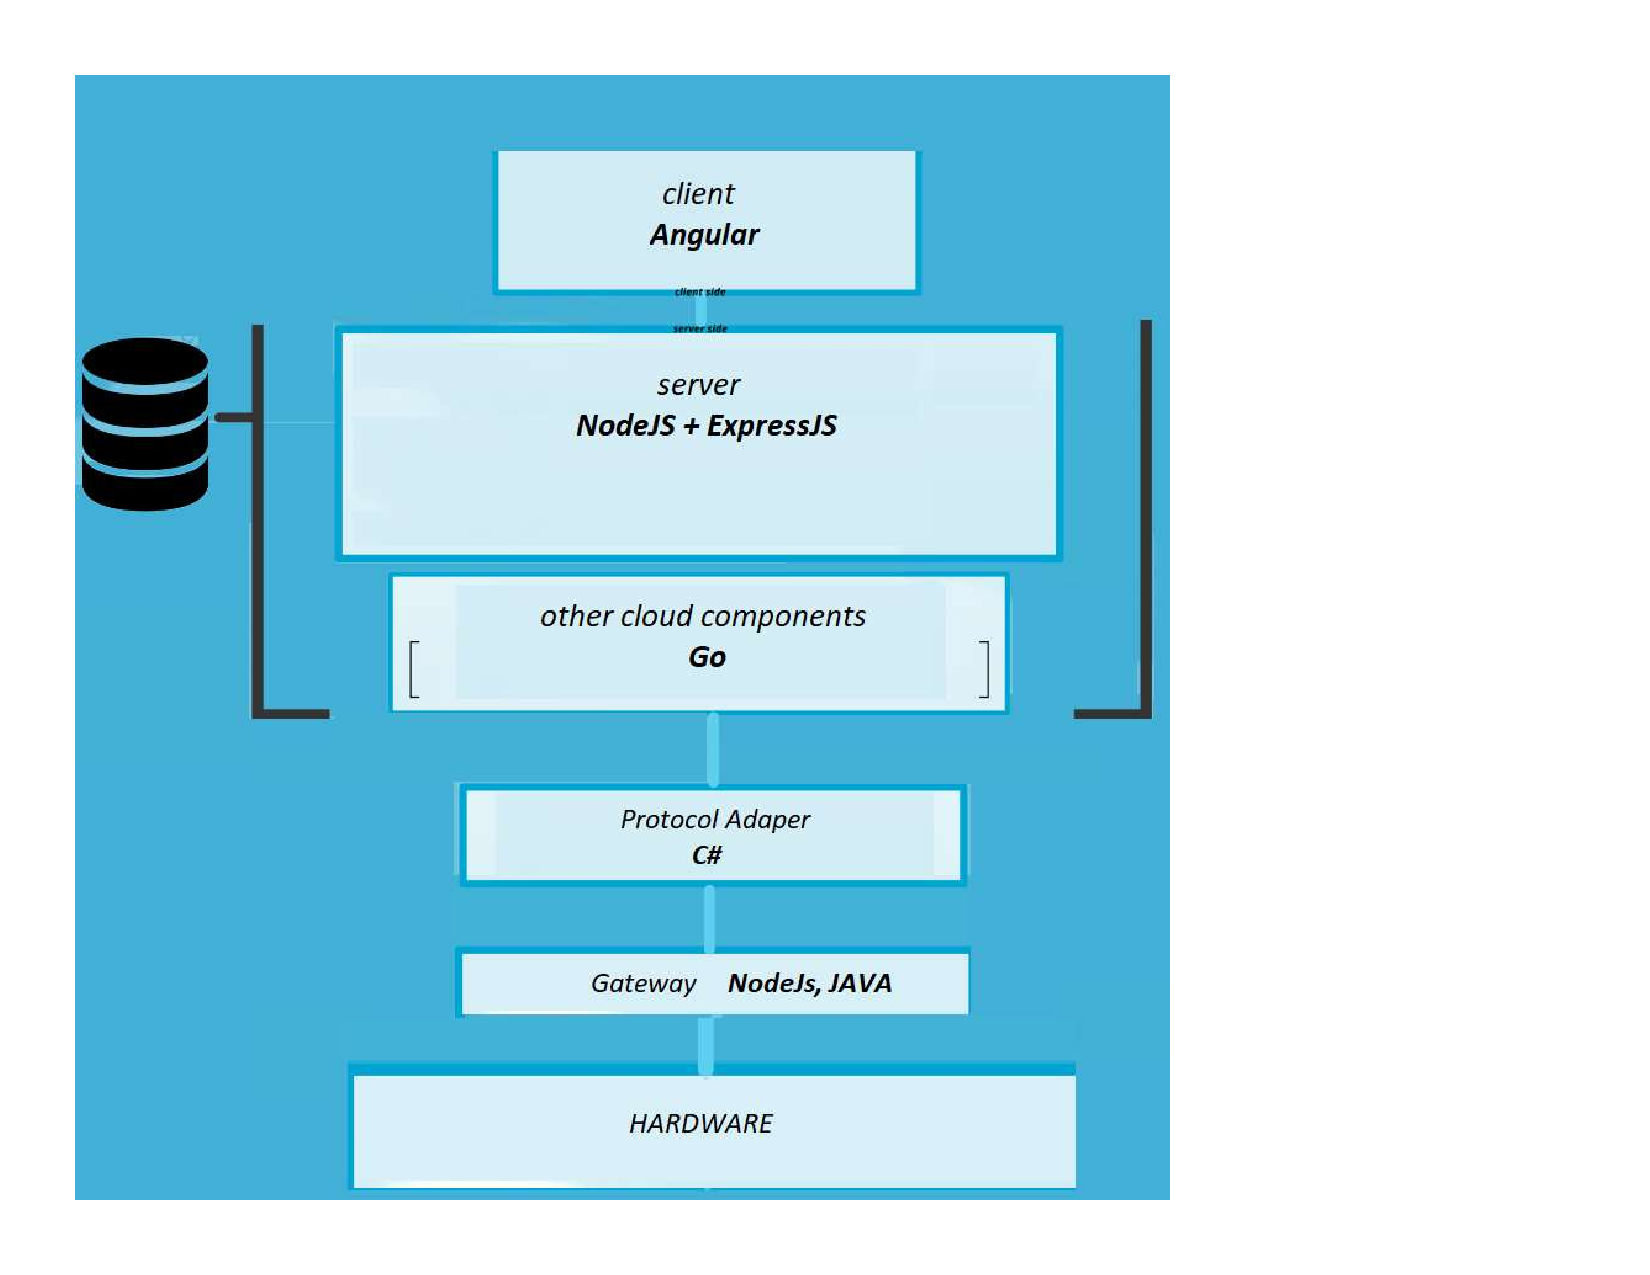
\includegraphics[width=0.70\textwidth,]{architecture.pdf}
	\caption{BOIC architecture}
	\label{fig:BOIC architecture}
\end{figure}

	\subsection{Description of the Continuous Deployment Environment }
	
	\begin{figure*}[!t]
		\centering
			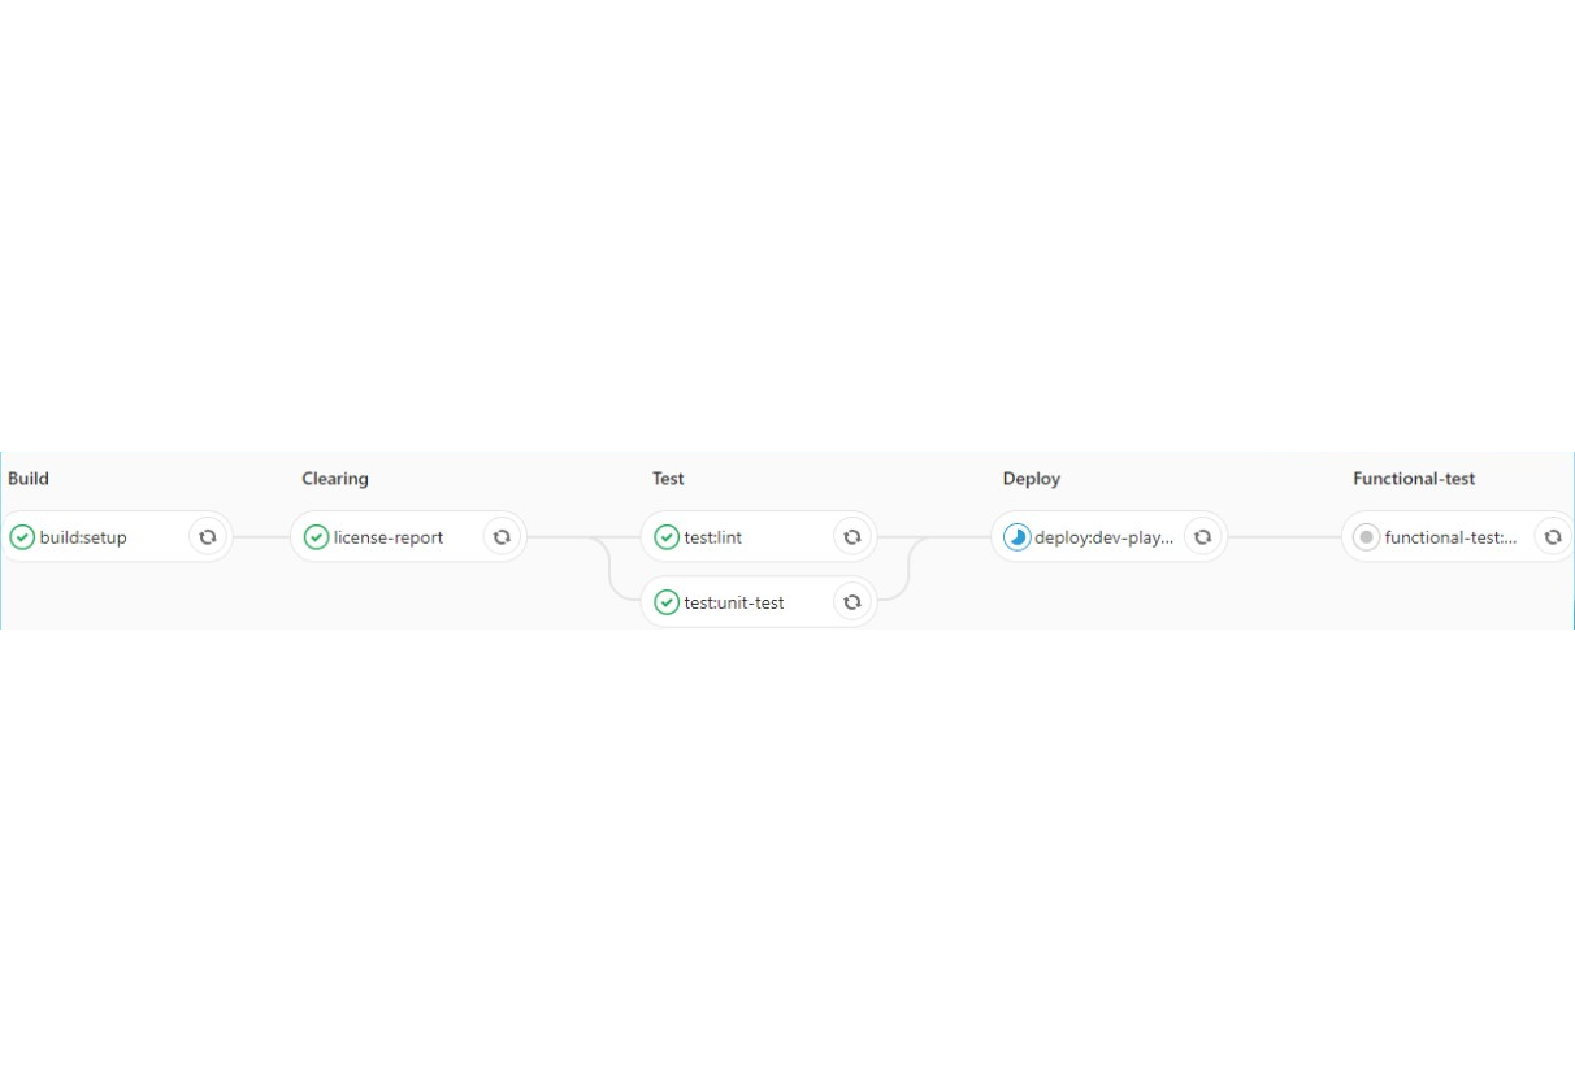
\includegraphics[width=1.00\textwidth]{UIpipeline.pdf}
		\caption{UI component pipeline}
		\label{fig:UIpipeline}
	\end{figure*}
	
	In a traditional configuration management scenario, there may be a plethora of servers needed for web development activities.
	Staging, committing, packaging the developed code, testing at each stage, source controlling and finally publishing at production server(s) may take place on a number of machines.
	This can end up in high costs of operation and maintenance in order to enable development activities.
	
	In cloud computing, utilizing containerization, each one of these development activities can be operated in a docker container.
	Figure~\ref{fig:UIpipeline} shows the GitLab pipeline for the UI component developed in Angular.
	GitLab is a continuous integration tool that supports the teams by hosting code repositories (similar to GitHub), providing defect tracking, enabling code reviews and continuous integration support. 
	Another example of a continuous integration tool is Jenkins, which can serve the same purpose thorough is extensions.


	The team uses Git for source control. \todo{about git}. 
	When any code is submitted, the application is built in a docker container, OSS Clearing for licensing is executed, unit testing and linting are done, the application is deployed to an cloud-hosted container and automated UI tests are run targeting this deployment.
	If testing passes, the code can get merged to the master branch. 
	This automated testing process ensures that after any code commit, the application is tested end to end and the quality is ensured. 
	
	To give a sense of scale, at the time of writing, the front end is over 15k lines of TypeScript code in Angular, over 1k lines of unit tests in Karma, over 4k lines of end to end (e2e) UI tests in Protractor. 
	There are over 200 unit tests that execute in seconds, over 300 e2e UI tests that execute under 10 minutes. 



\subsection{Description of the Test Code Structure}

	\subsubsection{Page Object Pattern}

	Released in 2011, Angular is popular front-end JavaScript framework for designing dynamic web applications.
	It is maintained by Google with the help of the open source community.
	It recommends the use of Microsoft's TypeScript language, which introduces class-based object oriented programming, static typing and generics. \todo{refer to wiki}.

	Components are the building blocks of Angular applications and they easily nest inside each other.
	Each component may have its own class, html and css file. This structure provides a way to design dynamic web applications while keeping the front-end code clean. 

	Page object pattern is a popular UI test automation design pattern in the industry. \todo{refer to Fowler and selenium paper}.
	In the spirit of Fowler's proposed terminology, we refer to web pages as 'pages' and Angular components as 'panels'.
	Each panel is a class. A page can be made up of many panels, which have a class-based object oriented structure.   

	Designing the test automation architecture, it became clear that it would not only be straightforward but also efficient to replicate the structure of Angular components in page objects as pictured in Figure~\ref{fig:angular}.
	One advantage of this is easier maintenance of the automation code as the development code changes.
	The other advantage is its benefits with asynchronous test execution.

	In a panel object, the element selectors become the class fields and the test actions become class methods within the component / panel.
	Enabling this class-based object oriented structure is TypeScript \todo{insert reference}
	TypeScript is a superset of JavaScript. It complies into JavaScript and includes the latest EcmaScript features \todo{reference to EcmaScript} .
	One of the recent advantages in the latest EcmaScript features is how it helps developers write sequential looking asynchronous code \todo{refer to async awaits}.

	With regards to test automation this means clean code that executes as fast as the environment allows, resistant to flakey tests and stale elements on the page. 
	This is because the page components load with panel-object-classes simultaneously, while the page element selectors get instantiated.
	We plan to study this design pattern in a future paper. For the purpose of the current study, it is sufficient to understand that all test relevant methods are housed in classes that represent panel objects / Angular components.
	
	\begin{figure}[!h]
		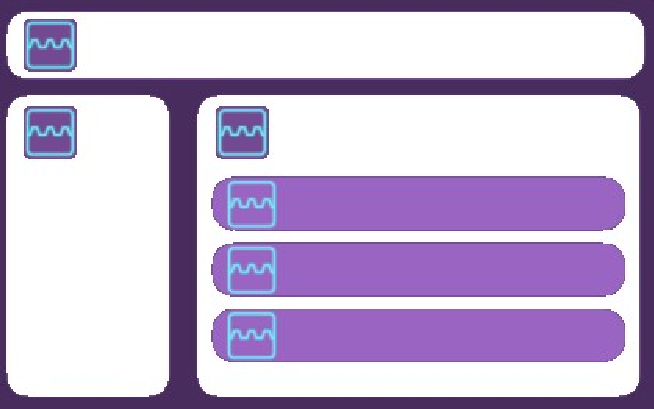
\includegraphics[width=0.45\textwidth,]{angular.pdf}
	\caption{Angular components as page and panel objects}
	\label{fig:angular}
	\end{figure}

	\subsubsection{Test data}
	The test data is stored in JSON files. This allows parameterization of test inputs, input-driven tests, as well as ease of maintenance as the UI changes.
	Another perk of using JSON is being able to convert test suites generated with CT tools - ex: ACTS, CTWedge \todo{references }- from csv format to JSON format.

	\subsubsection{Test Specifications}

	\begin{figure*}[!ht]
		\centering
			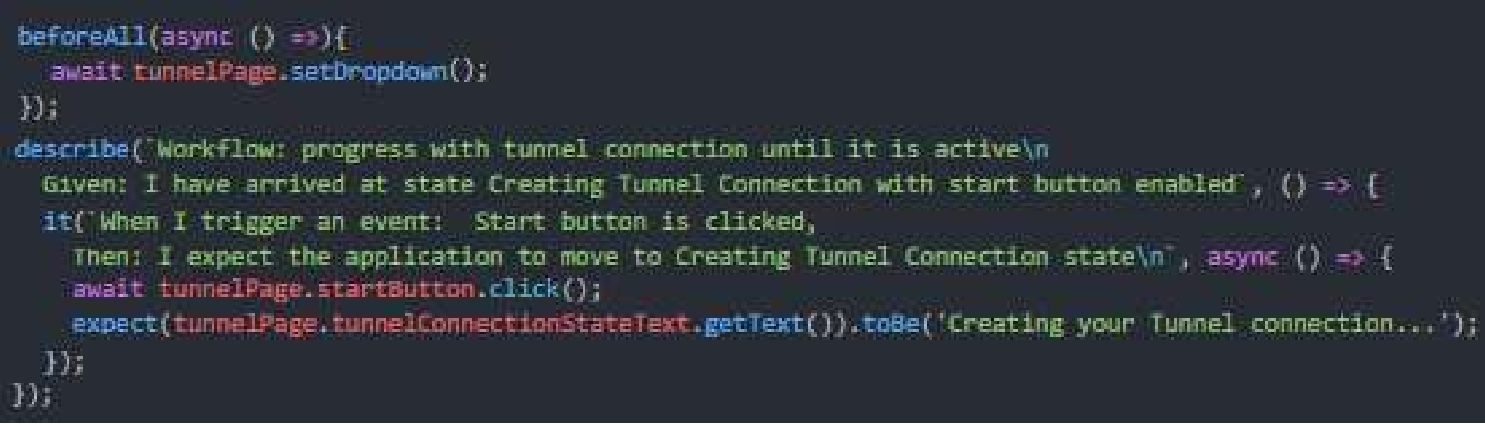
\includegraphics[width=0.90\textwidth]{codeSample.pdf}
		\caption{Protractor test code sample in State-based, Behavior-driven Acceptance format}
		\label{fig:codeSample}
	\end{figure*}	


	\begin{figure}[!b]
		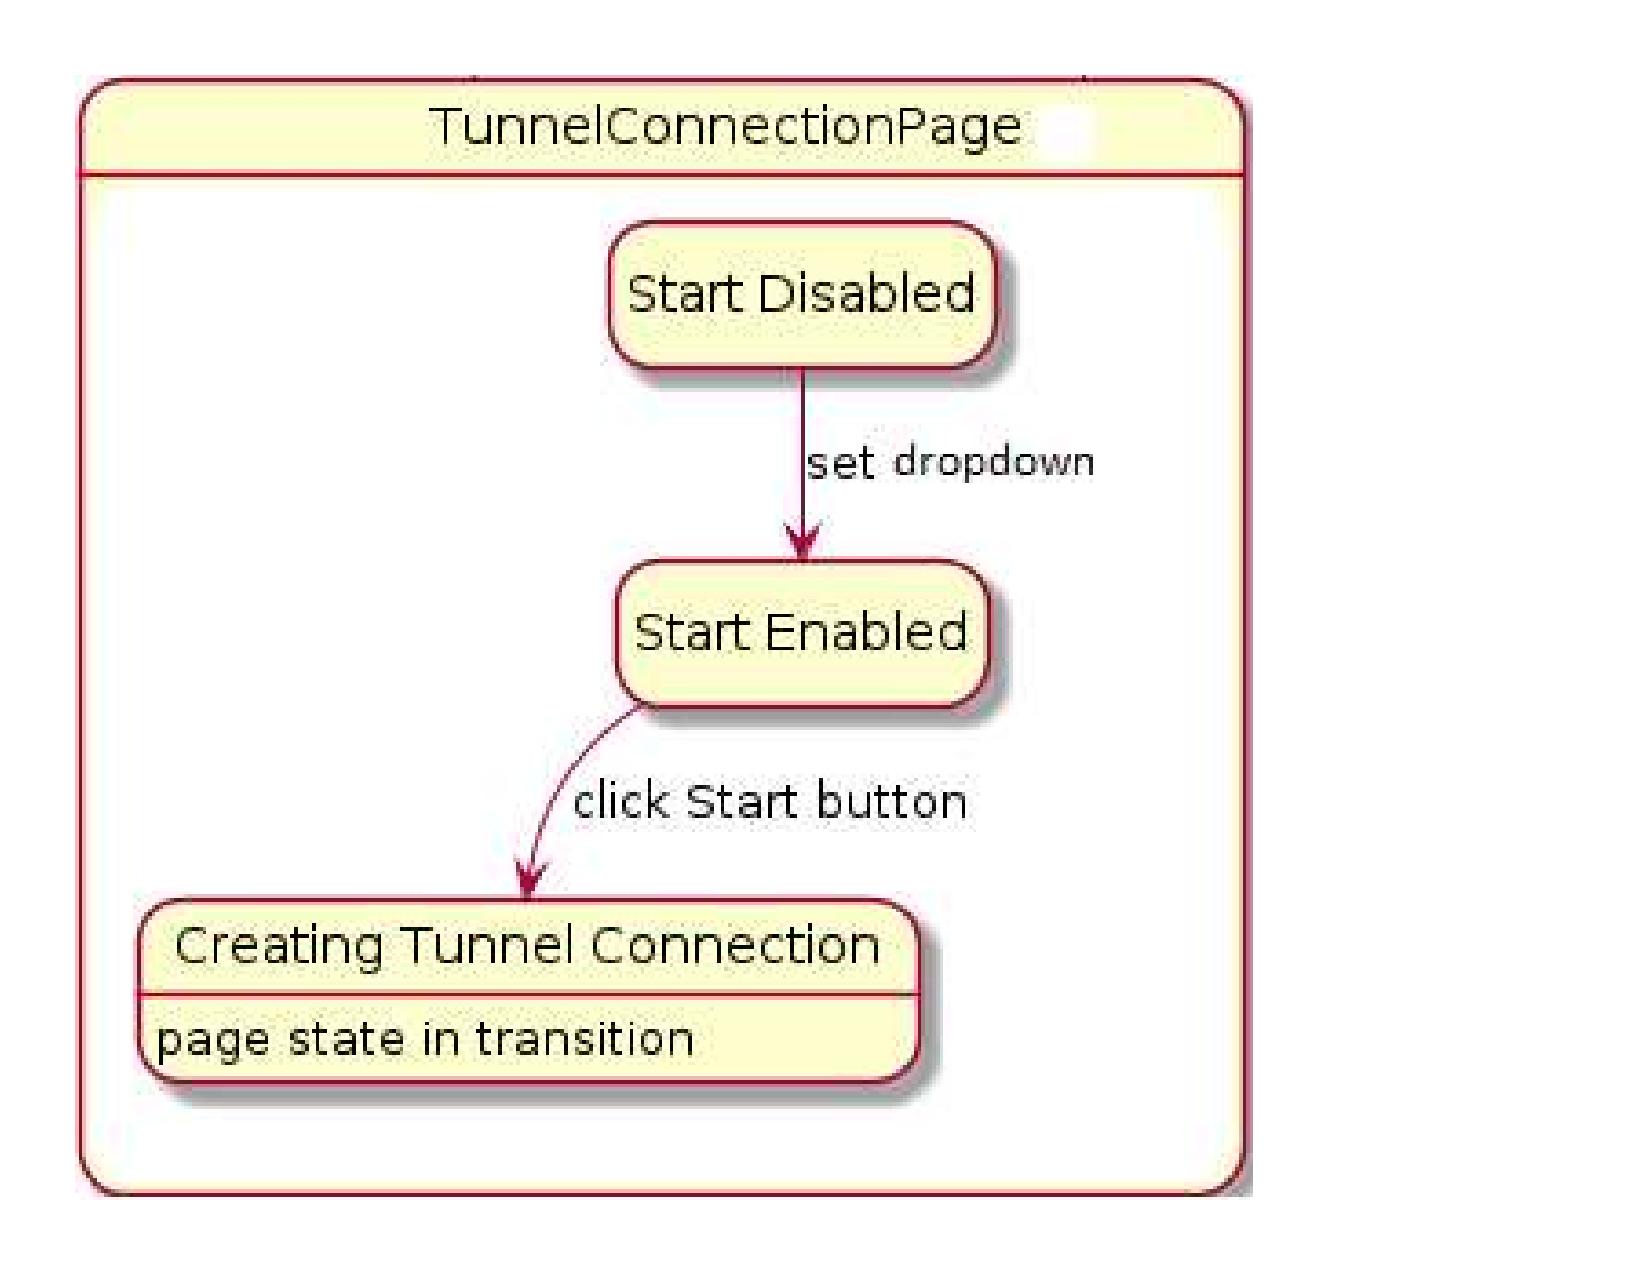
\includegraphics[width=0.60\textwidth,]{stateBasedScenario.pdf}
		\caption{State-based, Behavior-driven Acceptance Scenario}
		\label{fig:stateBasedScenario}
	\end{figure}

	The team uses Protractor test framework, which is the default end-to-end test framework for Angular applications. \todo{insert reference}
	It runs tests against the application running in a real browser, interacting with it as a user would.
	It combines technologies from Selenium webDriver, NodeJS and allows tests to be described in a BDD format -\textit{Given, When, Then}-, describing the overall behavior of a system at a low level.
	
	The test specifications are stored in Protractor spec files written in TypeScript. 
	The aforementioned benefits of the technology stack allow developers in test to write clean, simple, synchronous looking asynchronous code, without hard-waits or sleeps, resistant to stale elements and flakey tests.

	Over time during our development, the test specification came to be described in State-based, Behavior-driven Acceptance Scenarios \todo{reference blog post}. 
	Generally, these are in the format:


	\begin{itemize}
		\item [] \textit{Given I have arrived in some state} 
		\item [] \textit{When I trigger a particular event} 
		\item [] \textit{Then the application conducts an action}
		\item [] \textit{And the application moves to another state}
	\end{itemize}

	It was found out that this style of expression is not only descriptive at a meta level, but also maps well to the page object pattern.
	Figure~\ref{fig:codeSample} and Figure~\ref{fig:stateBasedScenario} show an a Protractor test spec sample with a state-based, behavior-driven acceptance scenario.
	
	As can be observed in the sample code from Figure~\ref{fig:codeSample}, \textit{tunnelPage} class / page-object is utilized for:
	
	\begin{itemize}
		\item [] - setup, using the \textit{setDropDown()} class method. 
		\item [] - test action, using the \textit{startButton} class field.
		\item [] - test assertion, verifying that \textit{tunnelConnectionStateText} class field / selector shows the correct text.
	\end{itemize}

	The code also samples the Protractor BDD style where a test workflow scenario is covered. 
	The \textit{it} block is one test in the workflow, the \textit{describe} block houses more tests / \textit{it} blocks that lead to the completion of the workflow - not shown in this example for the sake of simplicity.
	
\section{Test Methodology}
	
	In the following sections test designs using combinatorial testing techniques will be described. 
	Note that, this study will focus on black box test automation of the front-end. Testing at different levels of the architecture is planned to be studied in a future paper.

	For all combinatorial test suite generation CTWedge was used and for coverage measuring CAMetrics and CCM were used \todo{reference}.
	Traditionally, ACTS has been used in the organization during previous work.
	CTWedge and CAmetrics were preferred over their desktop contenders for a few reasons.

	\begin{itemize}
		\item [] - \textit{Portability and ease of use} : it is easier to copy a few lines of script and paste it at a url to generate a test suite in the case of CTWedge. It is also easier to upload a csv file to CAMetrics url and get a report quickly.
		\item [] - \textit{Ease of model modification} : it takes a few hours to master CTWedge scripting, but once done so, scripting proves to be a more robust interface to address changing test conditions; parameters, values or complex constraints. Comments in the script is an added benefit to readability. 
		\item [] - \textit{Cloud concept} : the entirety of the project is web-based and the web-based CT tools fit this concept.
	\end{itemize}
	
	\subsection{Input driven testing of hardware}

	\begin{figure}[!t]
		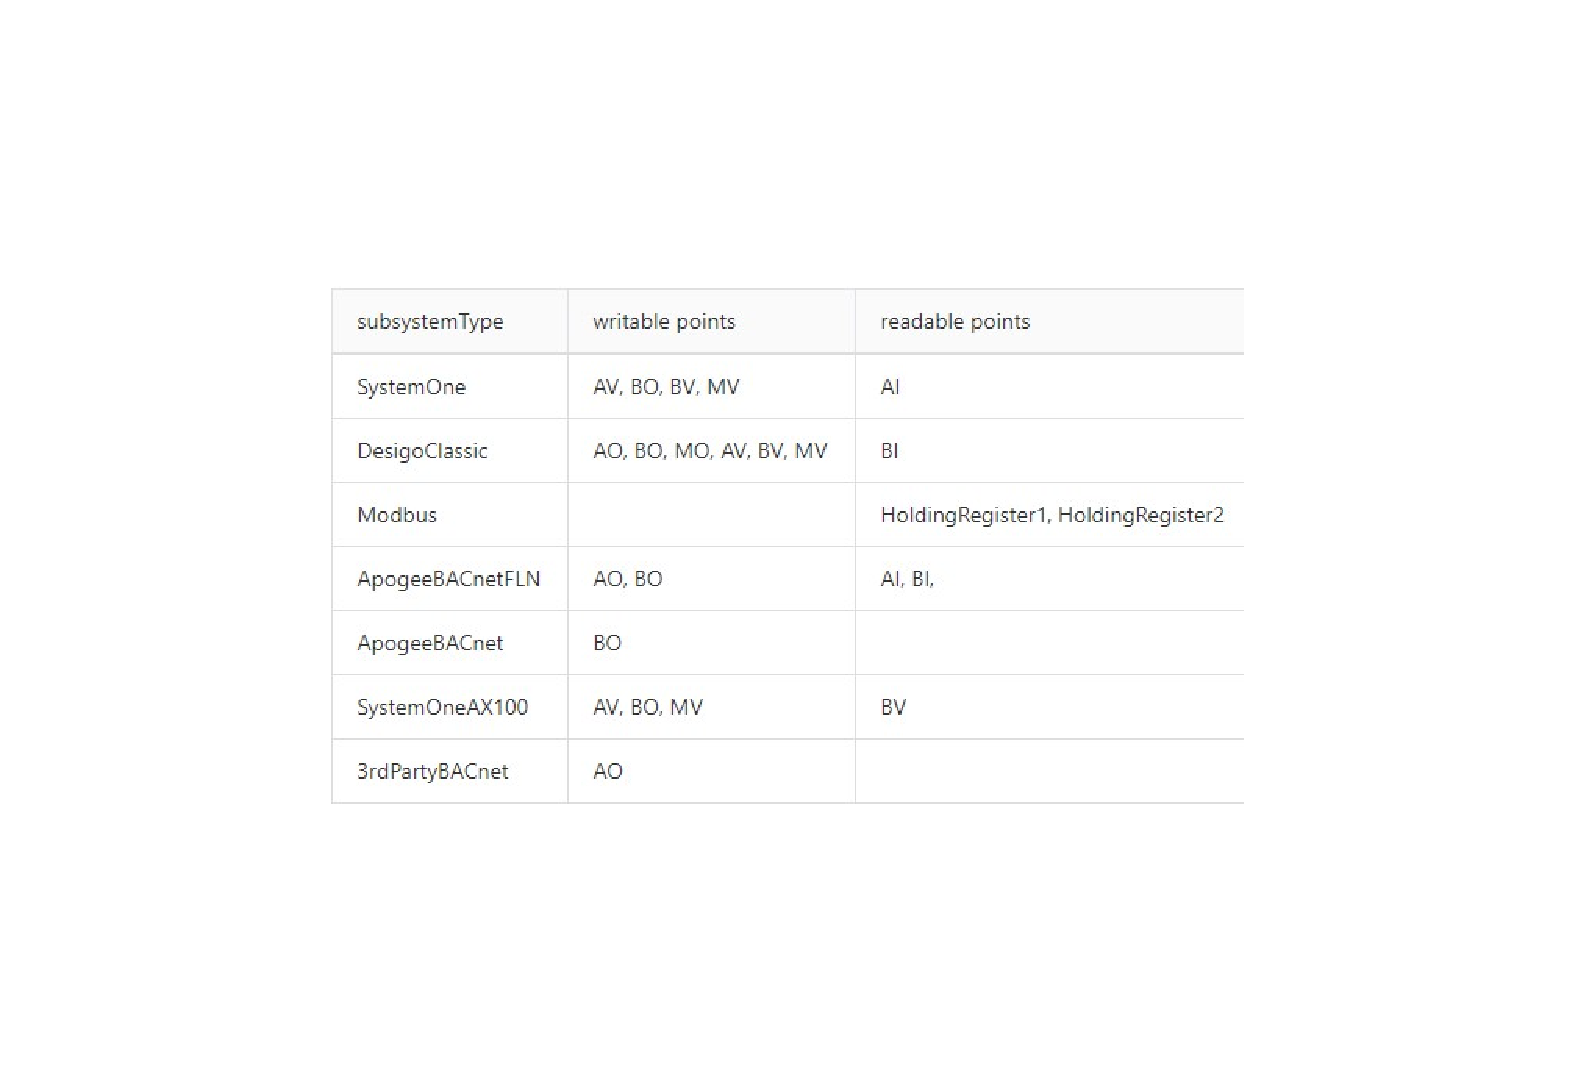
\includegraphics[width=0.50\textwidth,]{commandingIPM.pdf}
		\caption{Input Parameter Model for hardware setup}
		\label{fig:commandingIPM}
	\end{figure}

	BOIC provides widespread connectivity to legacy \& new controls, 3rd party, IoT and edge devices. The devices have no restriction to region; US, EU, Asia etc. 
	Consequently, the input parameter model (IPM) for the test setup needs to be agnostic to device types and control-points. This is achieved through parameters and values in JSON.
	Figure~\ref{fig:commandingIPM} describes the possible parameters for the hardware setup.

	The following code snippet shows how the input parameters and their values are represented in JSON. 
	For example, a binary-output point (BO) which may control a digital light or a fan -depending on context- may be referred to as \textit{FanCmd} (Fan Command) or \textit{LDO} (Logical Digital Output).
  Through parameterazation this complexity is abstracted. The test code only uses the parameters and the values of the parameters are easily manipulated depending on UI changes and or test configurations.

	\lstset{
    string=[s]{"}{"},
    stringstyle=\color{blue},
    comment=[l]{:},
		commentstyle=\color{black},
		tabsize = 2, %% Sets tab space width.
		showstringspaces = false, %% Prevents space marking in strings, string is defined as the text that is generally printed directly to the console.
		%numbers = left, %% Displays line numbers on the left.
		keywordstyle = \color{blue}, %% Sets  keyword color.
		stringstyle = \color{red}, %% Sets  string color.
		rulecolor = \color{black}, %% Sets frame color to avoid being affected by text color.
		basicstyle = \small \ttfamily , %% Sets listing font and size.
		breaklines = true, %% Enables line breaking.
		numberstyle = \tiny,
	}
	\begin{lstlisting}
		"SubSystemType": {
			"SystemOne": "DXR-VAV",
			"DesigoClassic": "DesigoClassic-ASG03",
			"Modbus": "Meter-DEM-1",
			"ApogeeBACnetFLN": "PTEC-Heat_Pump",
			"ApogeeBACnet": "PXC24-1",
			"SystemOneAX100": "RDY-Thermostat",
			"ThirdPartyBACnet": "Viconics"
		},
		"PointType_SystemOne": {
			"AV": "ECO CLG STPT",
			"BO": "FAN 1 SPD 2",
			"BV": "CMF BTN",
			"MV": "RM OP MODE",
		},
		"PointType_DesigoClassic": {
			"AO": "AS03'PTP'AnaObj'AO001",
			"BO": "AS03'Mis'CycTi'LED",
			"MO": "AS03'PTP'MulObj'MO001",
			"AV": "AS03'Ala'Per'AnaObj'AV001",
			"BV": "AS03'Ala'AsSta.DsavSta",
			"MV": "AS03'Ala'Per'MulObj'MV001",
			"BI": "AS03'PTP'BinObj'BI001",	
	\end{lstlisting}

	
	Figure~\ref{fig:modelCommanding} details the CT model scripted in CTWedge.
	It can be observed that the parameters \textit{subsystemType} and \textit{pointType} map directly from JSON data.
	On the other hand, parameters such as \textit{commandType} and \textit{commandToPointValue} represent abstracted test actions.
	All test actions are relaxed in the parameters and later, depending on the type of point, are restricted through constraints.
	Note that due to space restrictions, the model is shown partially and the complete version can be provided upon request.
	
	A constraint for Binary Outputs (BO) and Binary Values (BV) is scripted in CTWedge and would verbally translate as such:
	\textit{if pointType is BO or BV, you can only command it +1, -1, cancel, command type is fixed to OnOff and it's not readOnly}.
	
	A constraint for MultiState Outputs (MO) and MultiState Values (MV) is scripted in CTWedge and would verbally translate as such:
	\textit{if pointType is MO or MV, you can only command it +1 (and another), -1 (and another), cancel, command type is fixed to buttons3stages and it's not readOnly}

	Binary points and Multi-state points have two or more states, followed by confirm or cancel commands. 
	Certain points such as inputs may be \textit{readOnly} and do not have a commandType. Such points have a N/A value for \textit{commandType}, and the parameter is \textit{negated} through its use; a CT technique inspired by \todo{reference Rachel's paper}	

	Compared to  Binary and Multistate points, Analog points are more complex and have a variety of command options.
	They can be commanded via slider, text box, incremented or decremented. 
	They are prime candidates for boundary value analysis and equivalance partitioning in CT \todo{reference paper}.
	Partial script example for constraints can be viewed in Figure~\ref{fig:modelCommanding}. 
	It is our opinion that the test code snippet in Figure~\ref{fig:pointCommandingTestCode} will solidify the understanding of the application of constraints for analog points.

	\begin{figure}[!b]
		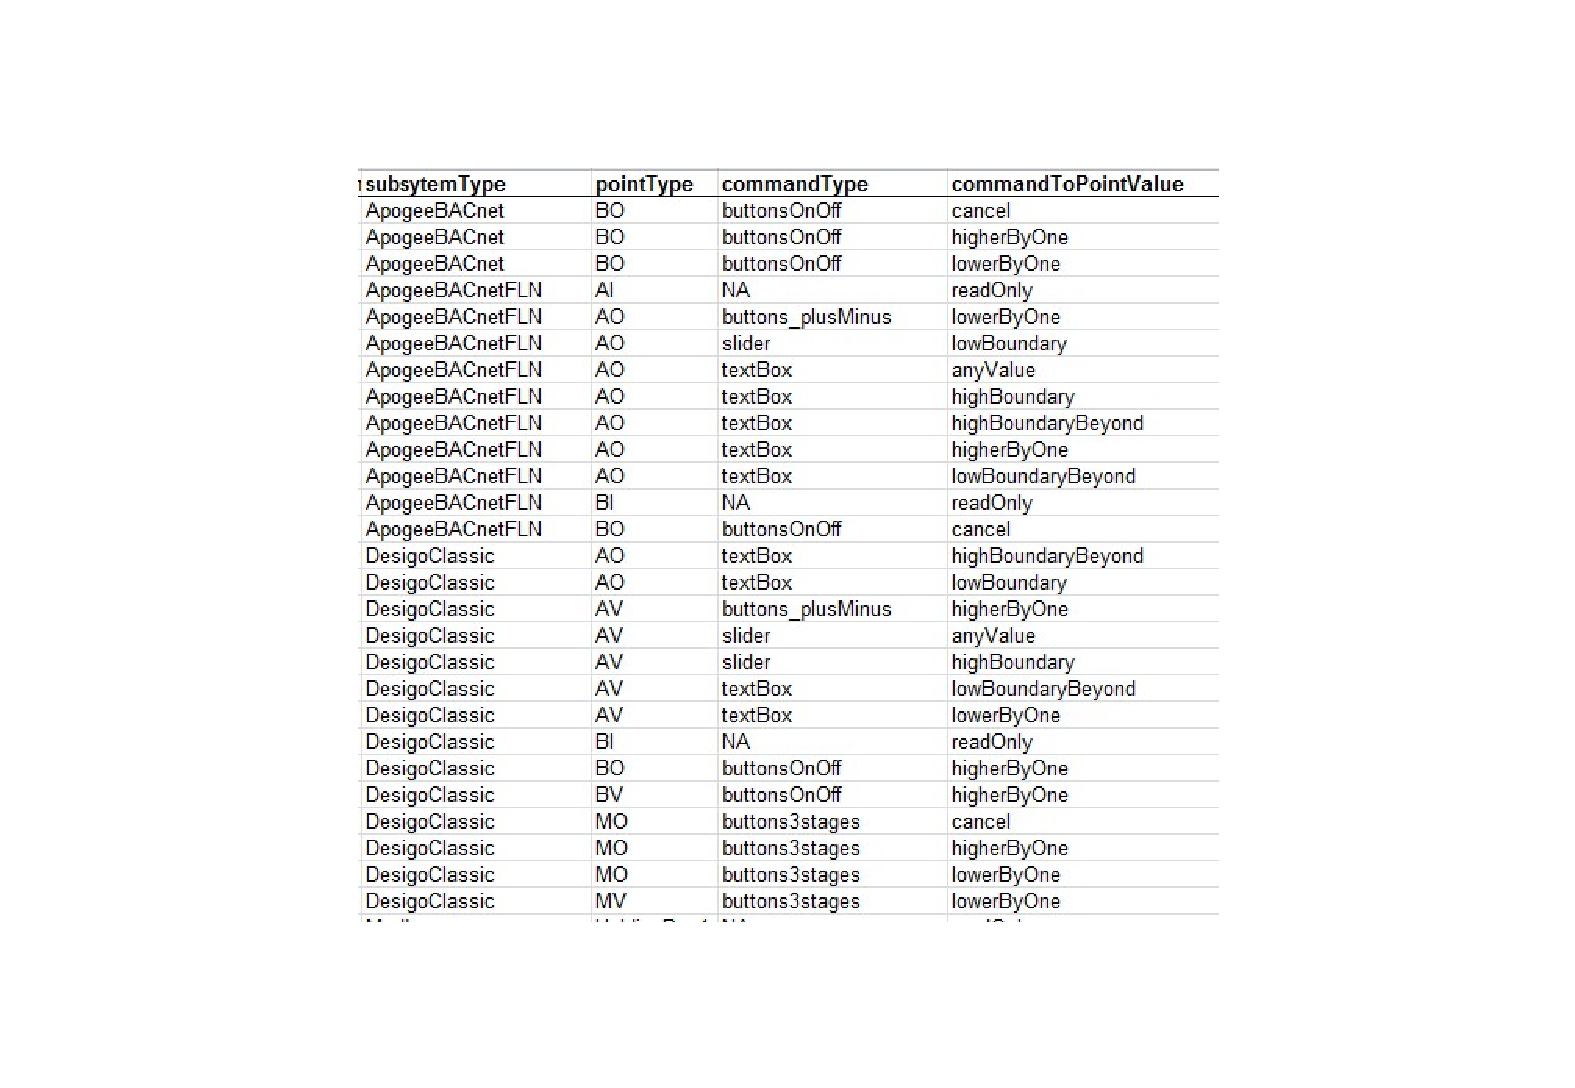
\includegraphics[width=0.50\textwidth,]{csvOutputCommanding.pdf}
		\caption{Input driven commanding test suite - partial}
		\label{fig:csvOutputCommanding}
	\end{figure}


	\begin{figure*}[!ht]
		\centering
			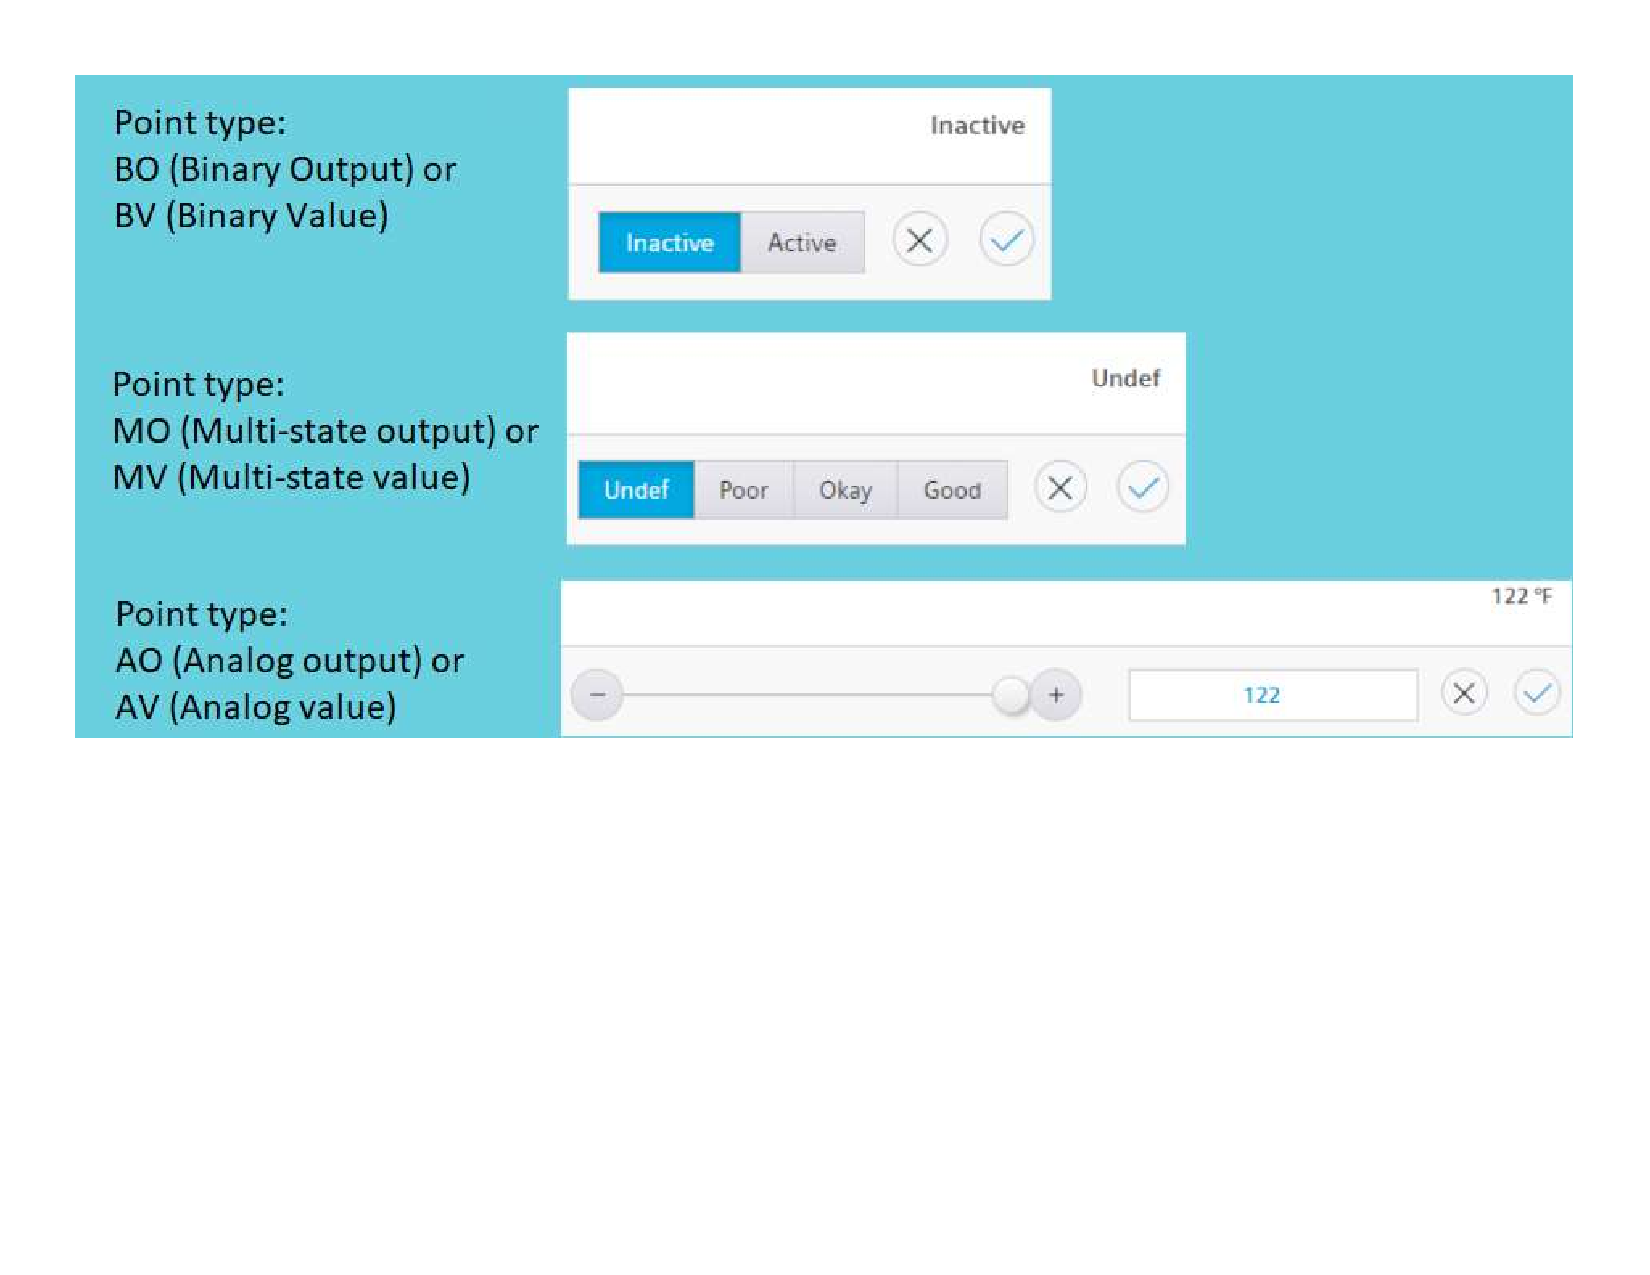
\includegraphics[width=1.00\textwidth,]{modelCommanding.pdf}
			\caption{CT model of panel and point commanding in CTWedge}
			\label{fig:modelCommanding}
	\end{figure*}


	The CT test design and test automation workflow is as such:
	\begin{itemize}
		\item [] - CT modeling of the IPM as in Figure~\ref{fig:modelCommanding}.
		\item [] - Generation of test suite in csv as in Figure~\ref{fig:csvOutputCommanding}, conversion into JSON as needed.
		\item [] - Based on the test suite, writing the automated test code as in Figure~\ref{fig:pointCommandingTestCode}.
	\end{itemize}

	\begin{figure}[!h]
		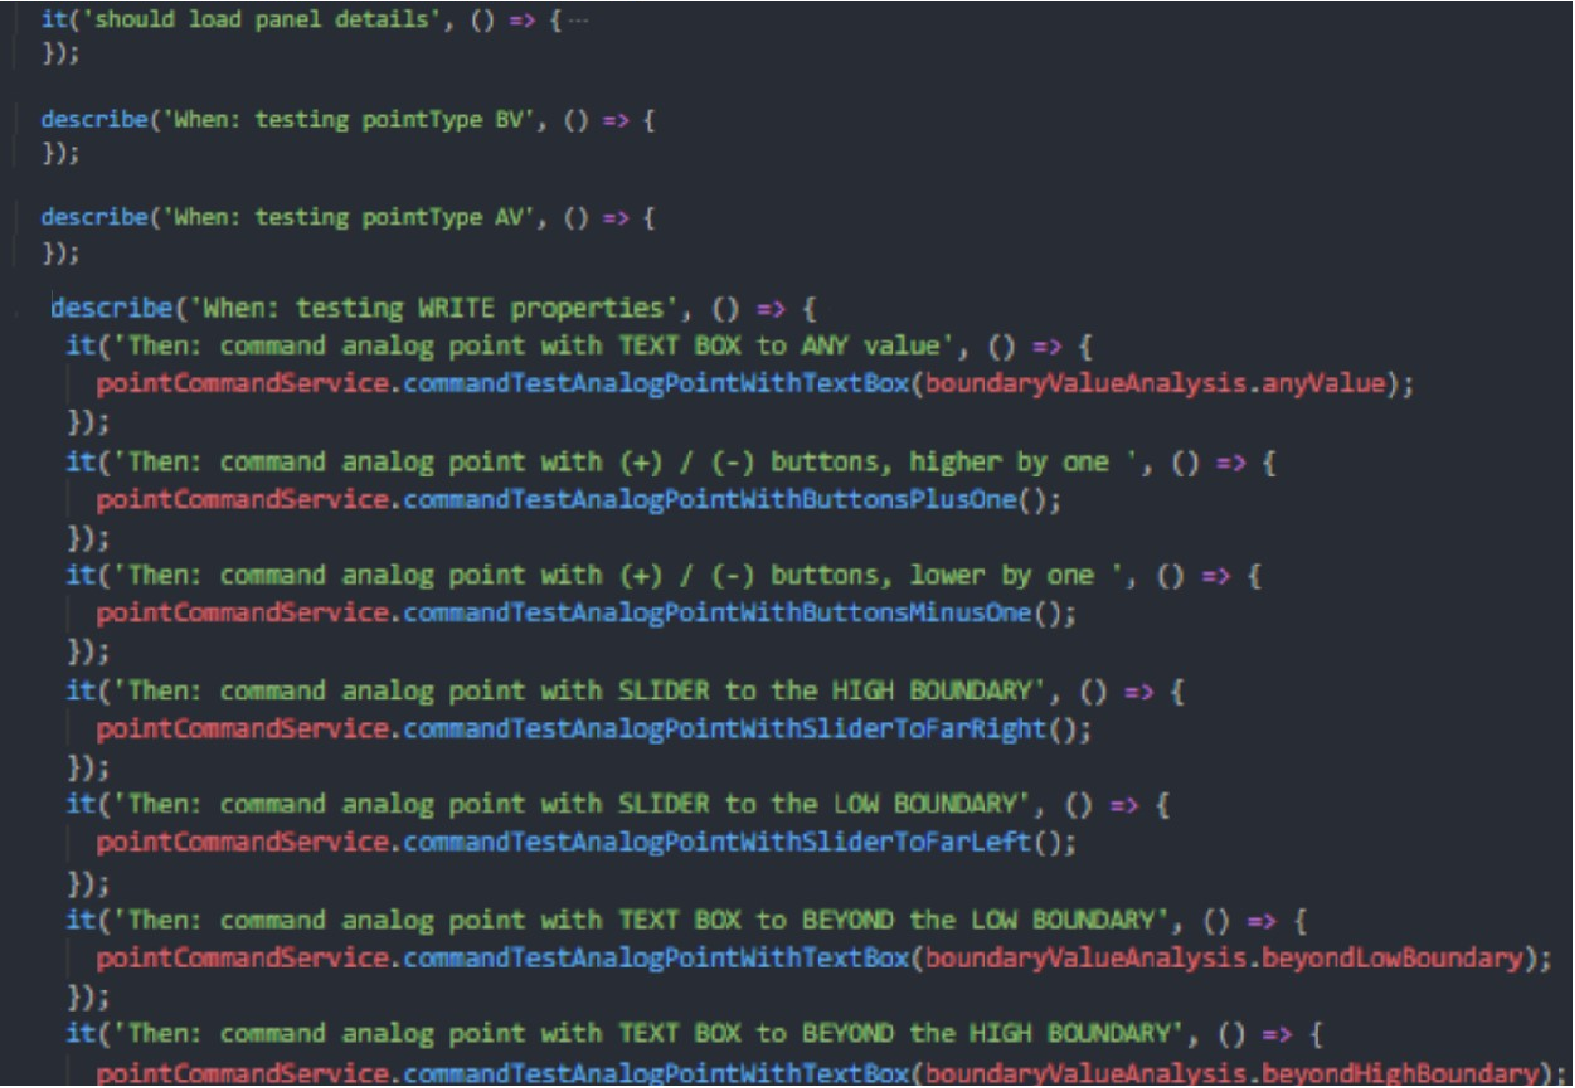
\includegraphics[width=0.50\textwidth,]{pointCommandingTestCode.pdf}
		\caption{Protractor \textit{describe} block for Analog Value point commanding in Desigo Classic panel}
		\label{fig:pointCommandingTestCode}
	\end{figure}

	Note that Figure~\ref{fig:pointCommandingTestCode} shows a part of the test spec in Protractor. 
	For ease of readability and confidentiality, test actions and assertions are handled under the functions in the code snippet. 
	For example the function \textit{commandTestAnalogPointWithSliderToFarRight()} does boundary value testing using the slider, and can be applied to any kind of analog point.
	Similarly the function \textit{commandTestAnalogPointWithTextBox()} continues boundary value analysis by passing in an integer to the text box, with a value greater than the boundary.

	\subsection{Filtering Points by Tag Combinations }

	In BOIC, tag filtering functionality is used to filter points in the system, by the devices the points are in.
	There are 13 possible tags, up to 5 tags can be chosen, tag choices cannot repeat, the final tag has only one tag choice, and there can be less than 5 tags for certain tag combinations if so is the nature of the points in the system.
	Figure~\ref{fig:tagFilterModel} displays an input parameter model of the functionality with a screen capture. 
	Note that due to space restrictions not all tags are displayed and only 2 blocks of 13 blocks of constraints are shown.
	
	Since the 5th tag is always a single choice, there is no need to represent it in the model and it is automated to be selected in the tests.
	The constraint logic is that no tag can repeat, with 4 constraints for each tag.
	For example one block of constraints is: \textit{if tag1 is 'cooling' then tag2 through tag 4 cannot be 'cooling', if tag2 is 'cooling' then tag 1, 3, 4 cannot be 'cooling'} and so on.
	CTWedge scripting provided cost savings while implementing the constraint logic. 
	Being able to copy the 4 lines of constraint logic, to replace the tag name, paste and repeat for each tag saved considerable amount of time.

	\begin{figure}[!h]
		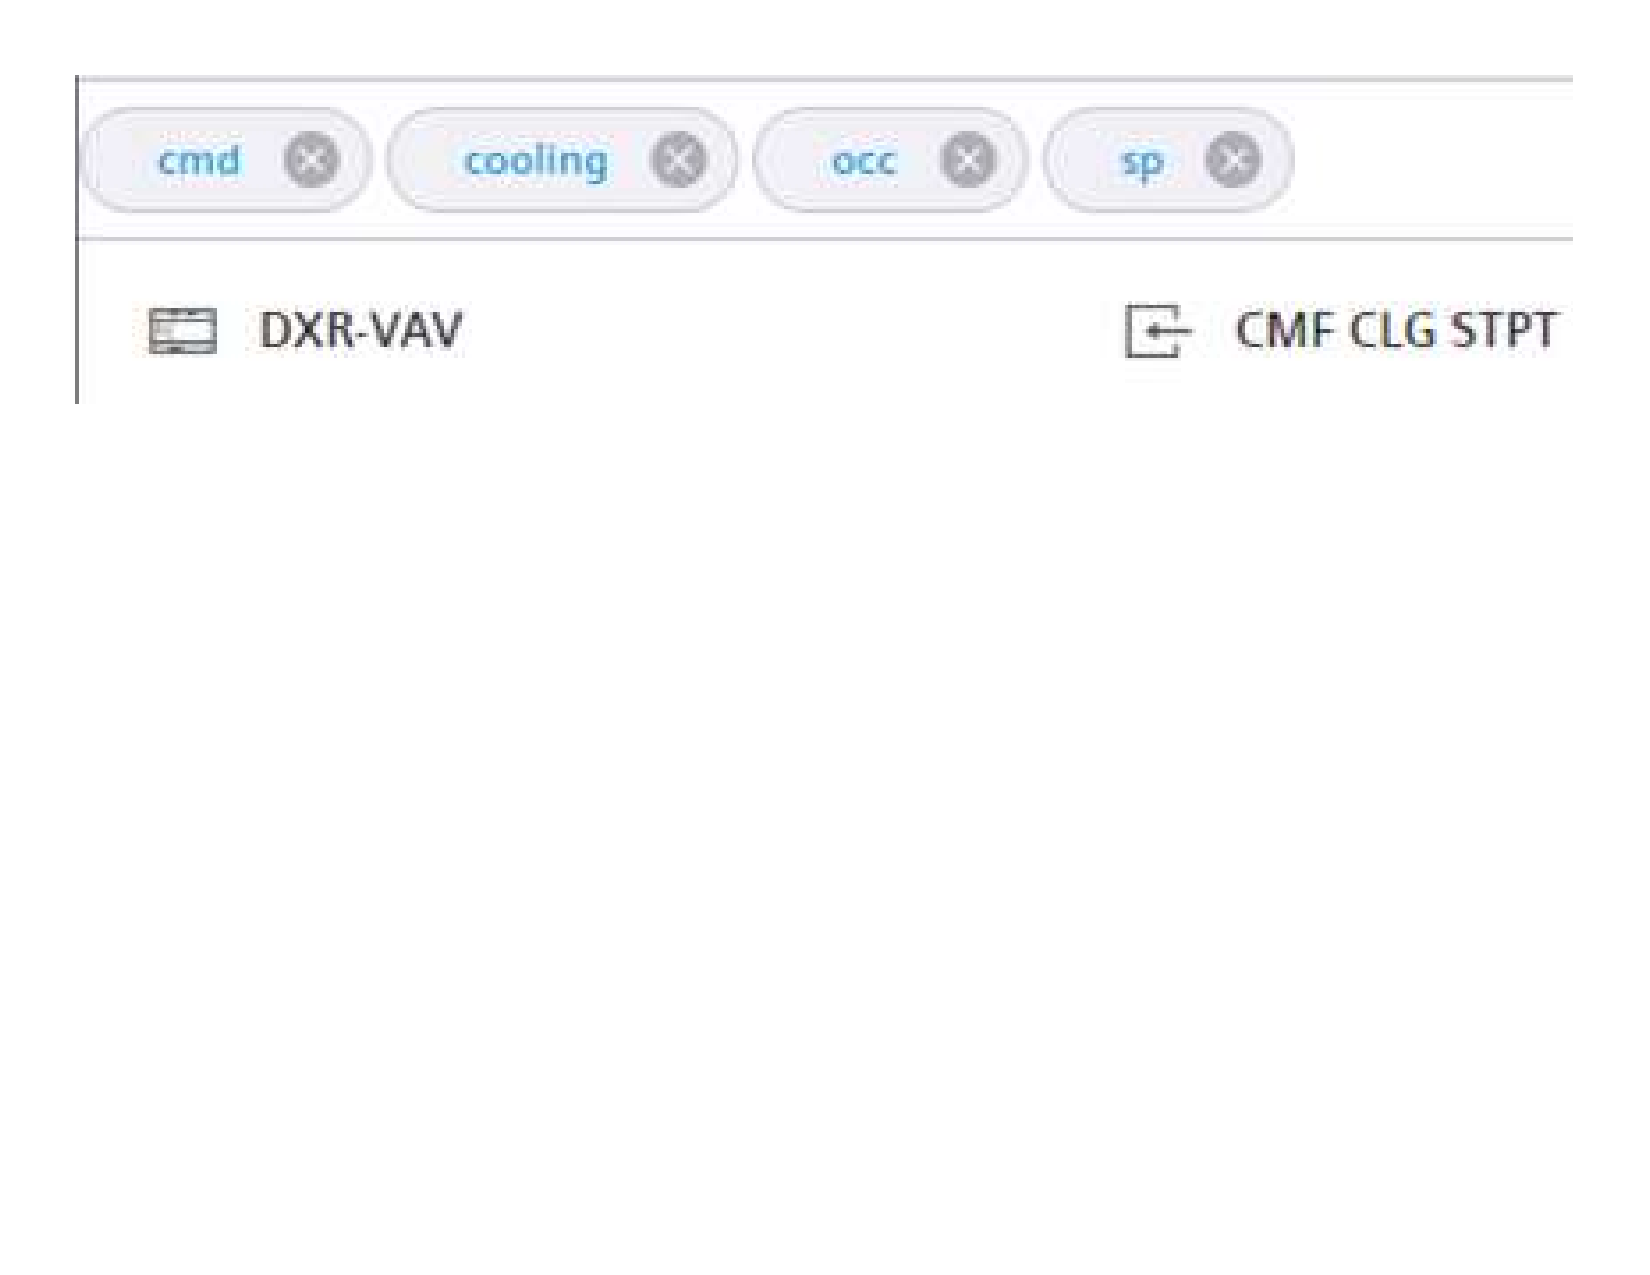
\includegraphics[width=0.50\textwidth,]{tagFilterModel.pdf}
		\caption{CT model of tag filtering in CTWedge}
		\label{fig:tagFilterModel}
	\end{figure}

	\begin{figure}[!hb]
		\centering
		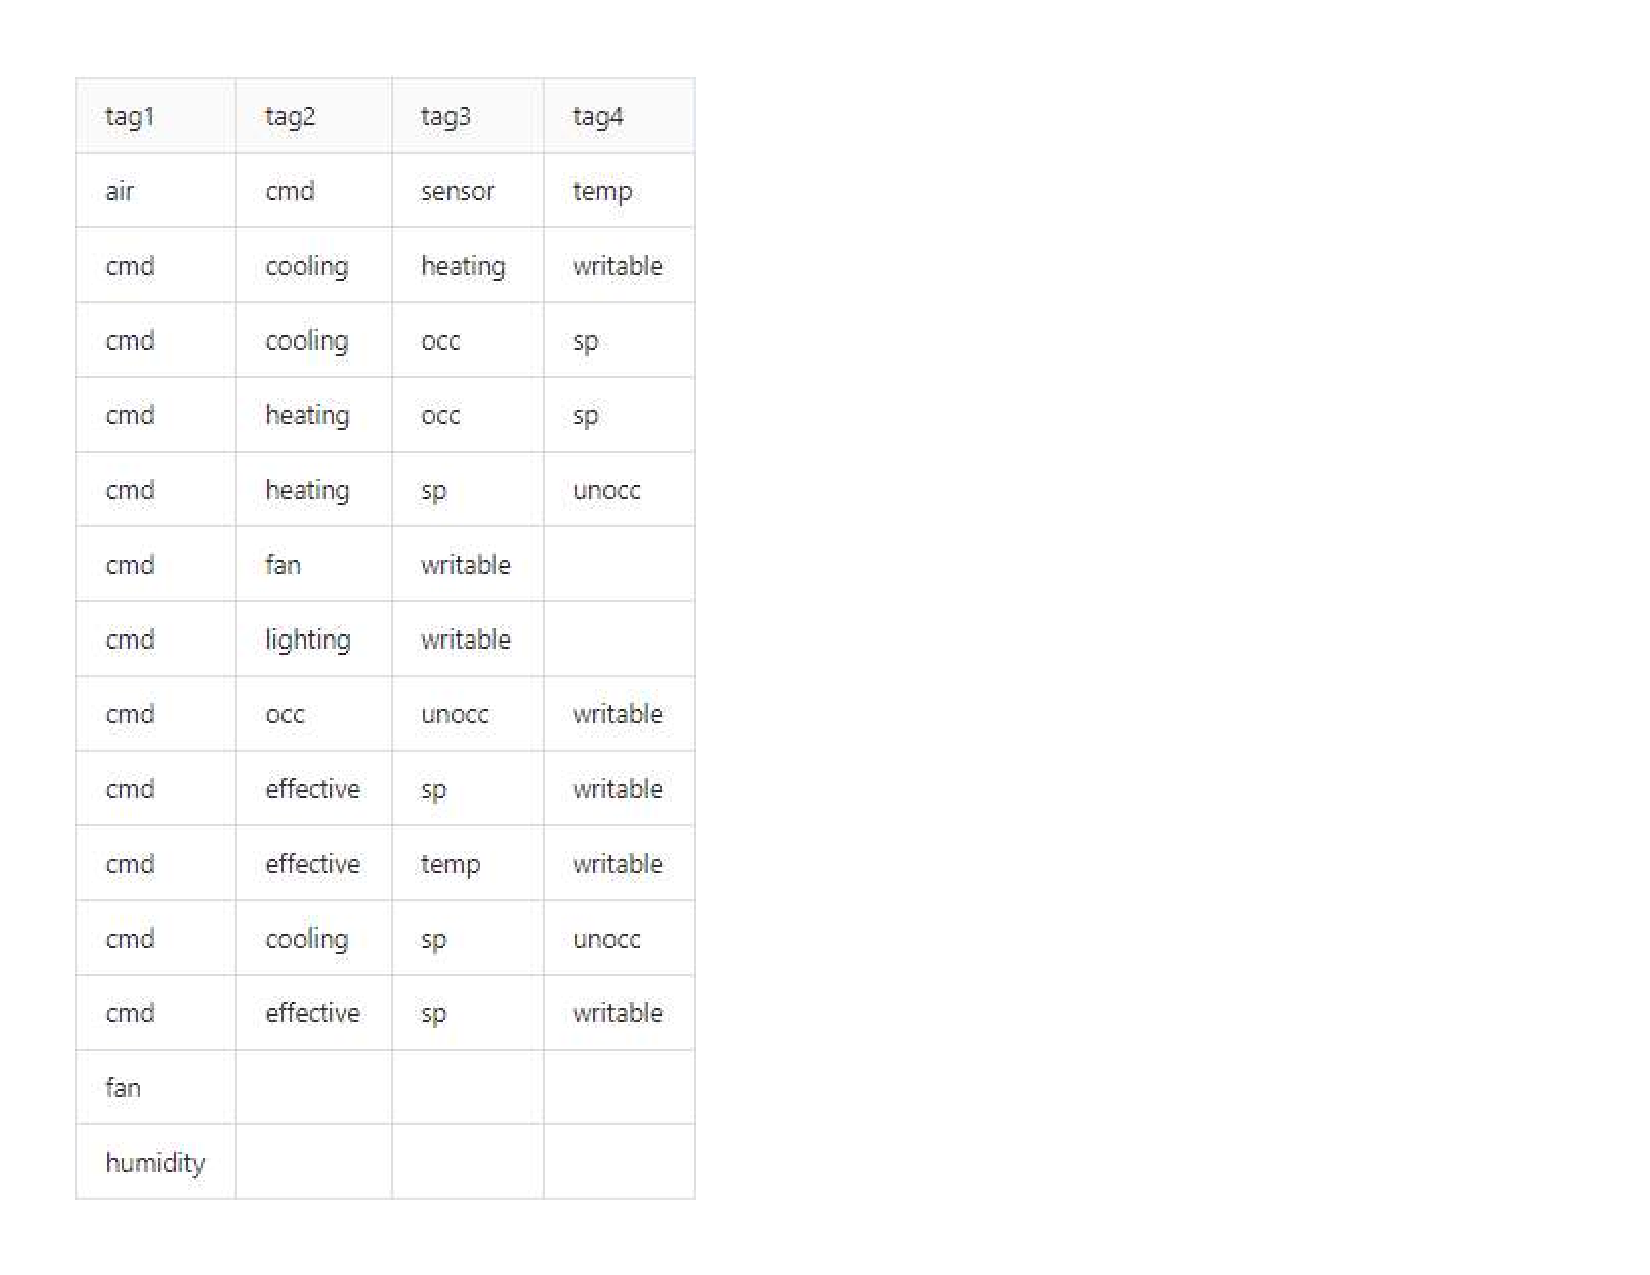
\includegraphics[width=0.32\textwidth,]{tagFilterCoveringArray.pdf}
		\caption{Covering array for tag filtering}
		\label{fig:tagFilterCoveringArray}
	\end{figure}


	With 4 parameters -final tag being default-selected due to a single tag choice being left in the tag dropdown menu- and 13 values each, the amount of tests generated could be vast. 
	However there were three factors that reduced the number of tests to the covering array of Figure~\ref{fig:tagFilterCoveringArray}:
	
	\begin{itemize}
		\item [] - 13 x 4 lines of constraint logic.
		\item [] - the final tag always being a single choice in the tag-dropdown menu. For example \textit{humidity} tag has 1 more tag choice available in the dropdown menu, but since it is a single choice it does not effect the number of tests.
		\item [] - certain points having only so many tags. For example any point with \textit{fan} or \textit{humidity} having a single tag (+1 tag), and certain combinations of tags - \textit{cmd} \& \textit{fan} or \textit{cmd} \& \textit{lighting} having at most 3 tags (+1 tag).
	\end{itemize}

	With the test suite of Figure~\ref{fig:tagFilterCoveringArray} generated, only one automation method had to be written and repeated for each test:
	
	\begin{itemize}
		\item [] - the method takes a single argument: a JSON parameter with a predefined string of delimeted tags. For example \textit{tagTest1 = "air,cmd,sensor,temp"}. 14 varieties, one for each test. These are infinately flexible, simply a different string can be passed in for a different set of tags.
		\item [] - in the method, the string of tags get split by the delimeter. Using these tags, the tag selection is done in an asynchronous for loop. 
		\item [] - as the tags are selected, the panel \& point combinations get filtered. The tag details of the points are verified to match the tags chosen in the filter.
	\end{itemize}

	

	\subsection{Sequenced Filtering, Searching, Sorting of Geo-located Sites}

	BOIC is designed so that the building operater can control a number of geo-located sites. 
	Each site has a unique address. The building operator has the ability to filter and sort the sites they have administration over:

	\begin{itemize}
		\item [] - Sites can be filtered by their status: \textit{Working Well, In Alarm, Disconnected}: 3 boolean states.
		\item [] - Sites can be filtered by any string entered in the text box.
		\item [] - Sites can be sorted by \textit{Status, Name, Street, Country, Creation Time}
		\item [] - The above actions can happen in any order and should give the same resulting list of filtered and sorted sites.
	\end{itemize}

	Figure~\ref{fig:siteFilterModel} shows the alarm filtering menu as well as the search text box and sorting buttons. 
	Alarm filters are modeled as 3 boolean states and the resulting covering array includes 4 configurations. 
	This result is plugged in to the next model, a technique from \todo{refer to your own paper} to reduce the number of tests and still provide cost effective coverage.
	The parameter \textit{filter-workingWell-inAlarm-disconnected} includes the the 4 configurations of these checkboxes as values. 

	The \textit{search} parameter is a text-box, which is open ended. For this, possible values were contemplated to be any string, address fields.

	The \textit{sortBy} parameter simply replicated the names of the columns. 
	In order to keep the number of tests low, instead of being a parameter in the model, reverse sorting of columns got covered in each automated test.
	This was also utilized as a setup \& cleanup in tests since sort order of the previous column gets retained; not utilizing this behaviour would cause tests to be non-modular.

	In order to have a deterministic test oracle, an array of sites were generated with varying data parameters - all stored in JSON - so that after filtering by site status and a search string, there would be at least 2 sites to test sorting with.
	
	Generating the tests, it was promptly realized that if sorting sites by column - possible values being \textit{Status, Name, Street, Country, Creation Time} - matches the search string -possible values being fields of an address - sorting became redundant and had no effect.
	These redundancies were addressed by adding constraints, for instance \textit{if sorting sites by Street, search string cannot be street name}. 
	CAMetrics was used \todo{reference to CAMetrics} to measure pairwise coverage gain per test: Figure~\ref{fig:coverageGainPerTest} and Figure~\ref{fig:coverageGainPerTest_withConstraints} show coverage before and after constraints being applied.
	The constraints eliminated 5 redundant test cases and the end result became a test suite of 19 tests. With this, a 20.8\% cost savings was achieved while developing automation test code.
	
	Finally the sequence of the user actions needed to be addressed. Previous research on this topic has been vast and is referred to in section \todo{insert section} .
	The two filtering operations and the sorting can happen in any order, and there 6 possible ways of ordering them.
	If the sequence of the 3 actions \textit{filter, search, sort} were represented as 3 parameters \textit{filterBeforeSearch, searchBeforeSort, filterBeforeSearch}, they could be simplified as \textit{AbeforeB, BbeforeC, AbeforeC}.
	Figure~\ref{fig:sorting} displays this logic in a table.
	As observed, case 1 and case 6 are impossible; if \textit{AbeforeB} and \textit{BbeforeC} have the same boolean value, \textit{AbeforeC} has to match that value.
	This logic of sequence was addressed with 2 constaints:

	\begin{itemize}
	\item [] \textit{if filterBeforeSearch is TRUE \&\& searchBeoreSort is TRUE then filterBeforeSort is FALSE}
	\item [] \textit{if filterBeforeSearch is FALSE \&\& searchBeoreSort is FALSE then filterBeforeSort is TRUE}
	\end{itemize}

	\begin{figure}[!t]
		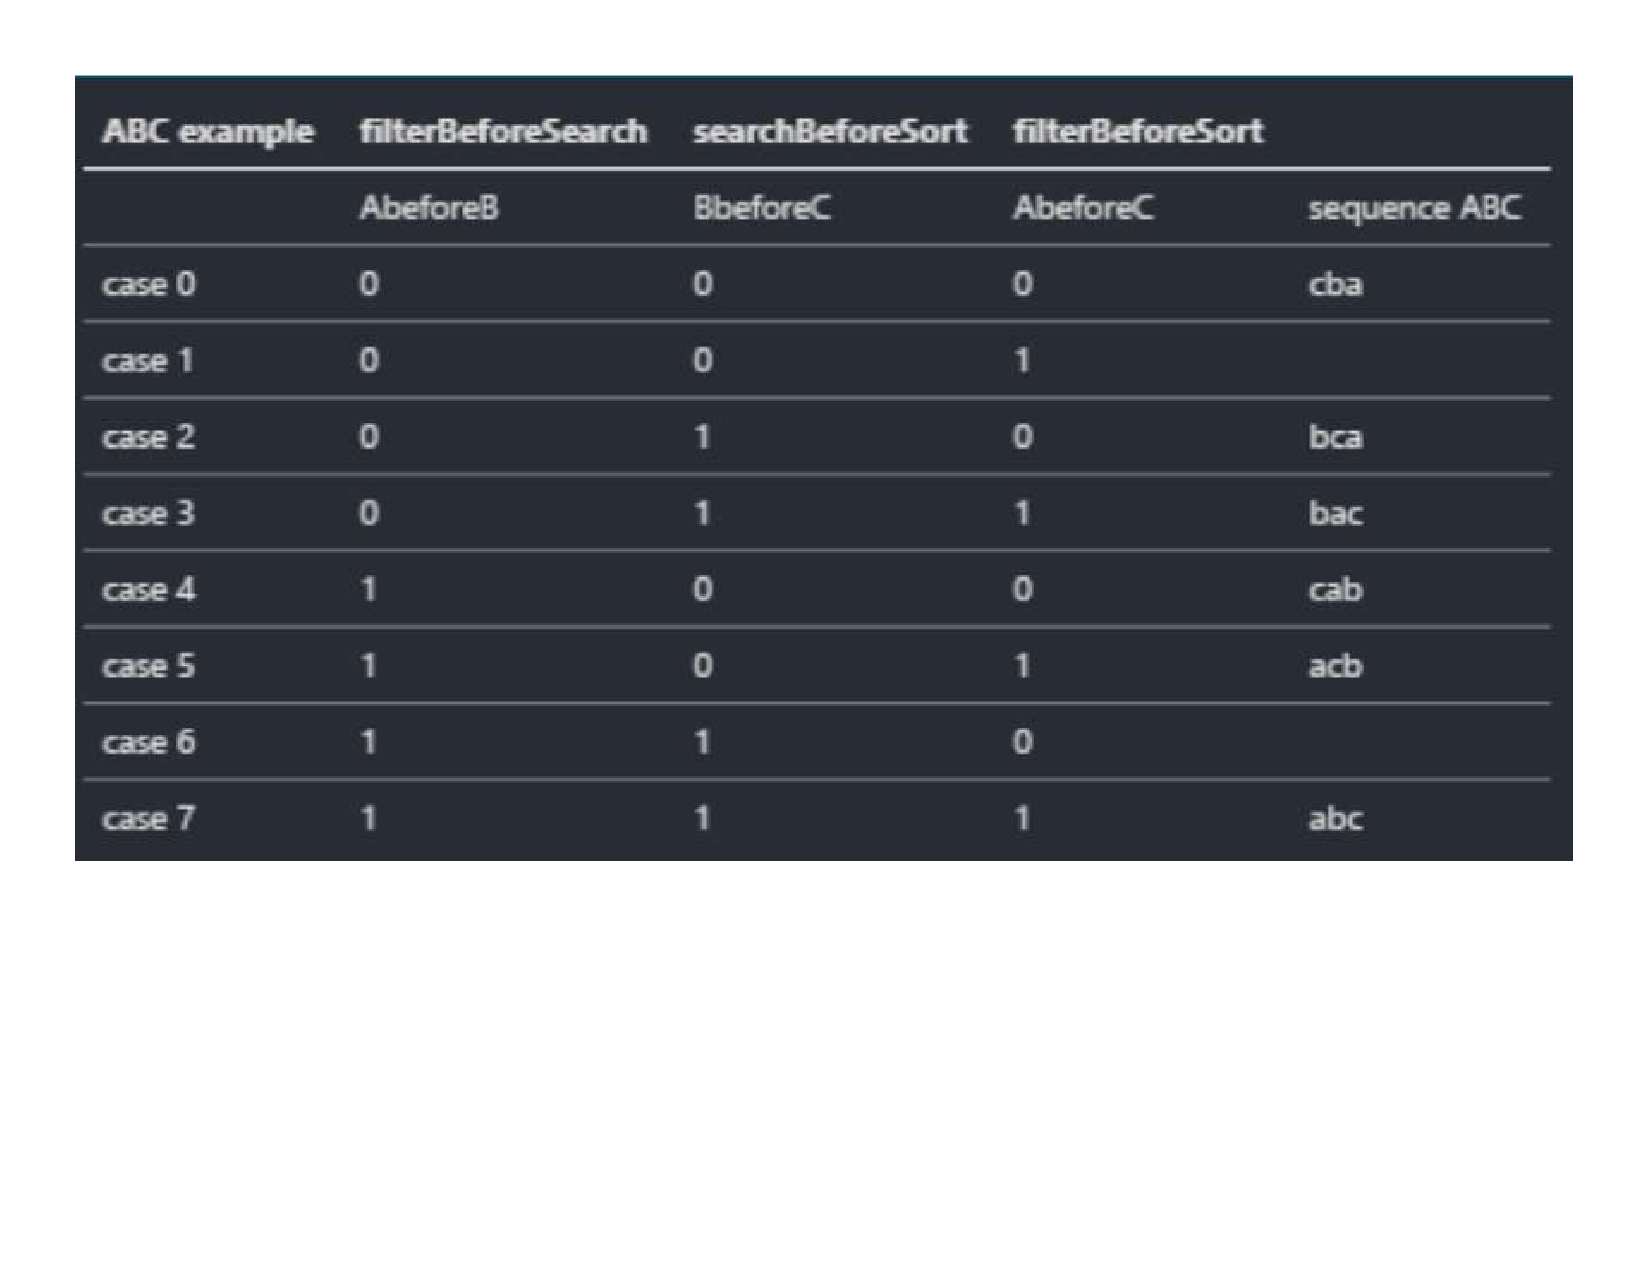
\includegraphics[width=0.50\textwidth,]{sorting.pdf}
		\caption{sequences of test actions}
		\label{fig:sorting}
	\end{figure}

	\begin{figure}[!h]
		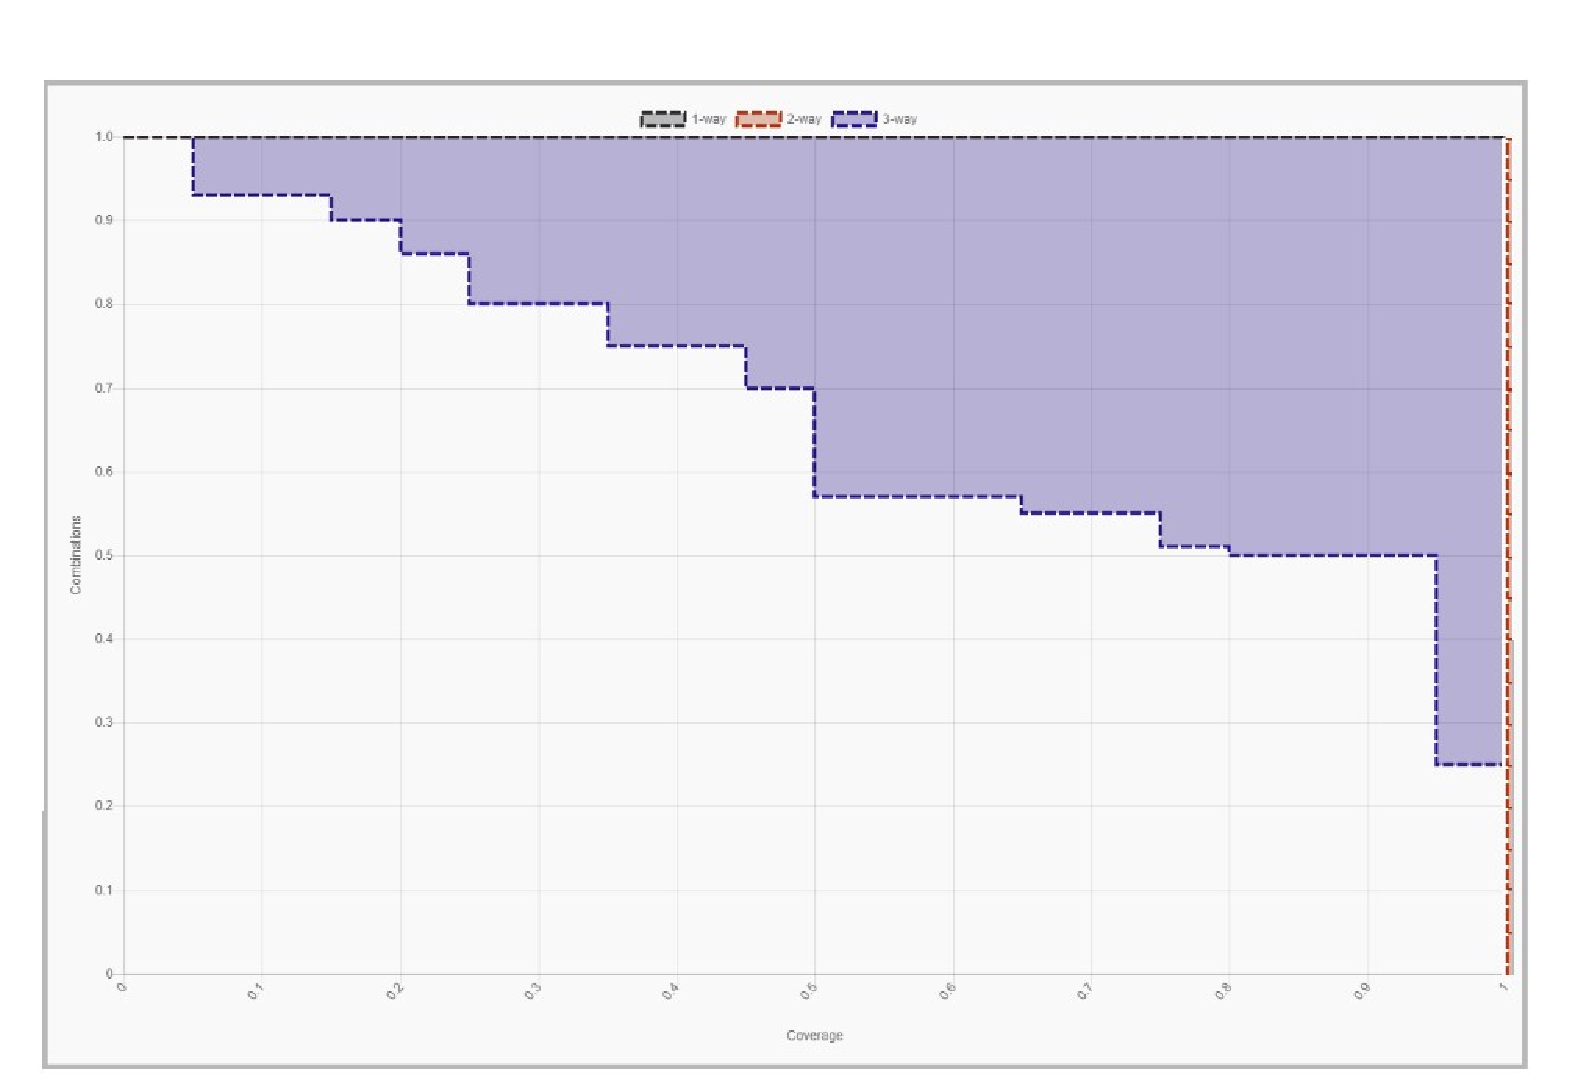
\includegraphics[width=0.50\textwidth,]{CompletenessCoverage.pdf}
		\caption{2-way and 3-way completeness coverage, measured with CCM}
		\label{fig:CompletenessCoverage}
	\end{figure}

	\begin{figure}[!h]
		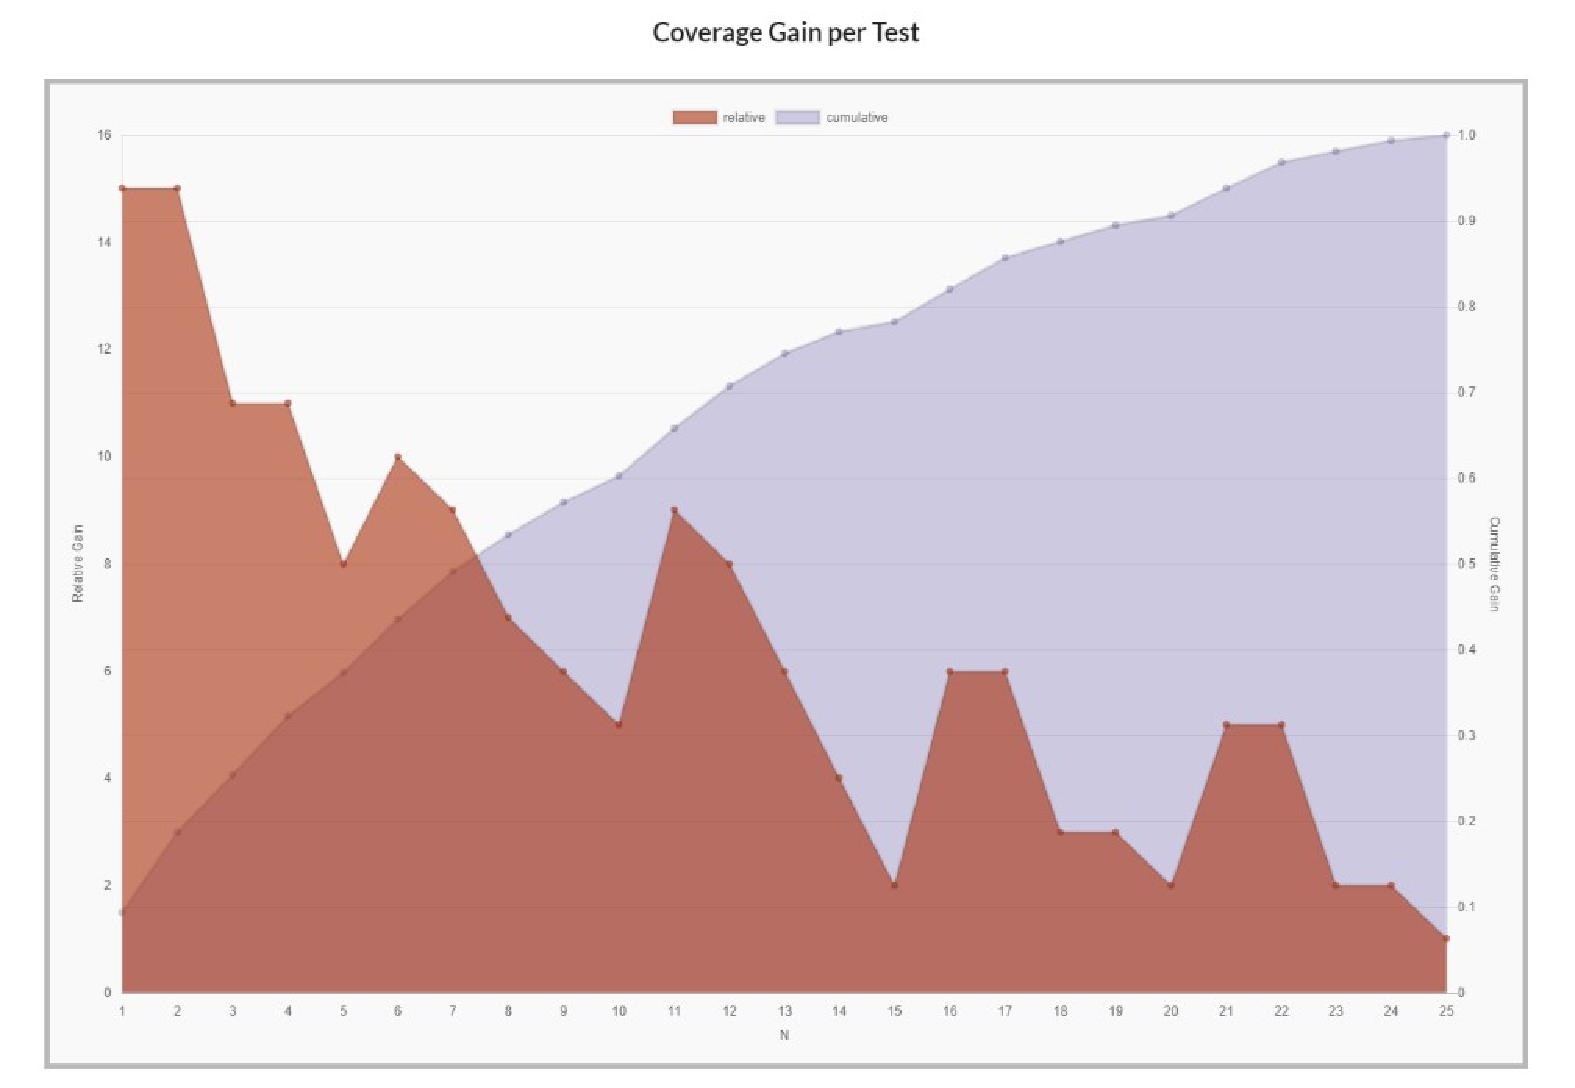
\includegraphics[width=0.50\textwidth,]{coverageGainPerTest.pdf}
		\caption{No constraints : relative gain (red) vs cumulative gain (blue) per test}
		\label{fig:coverageGainPerTest}
	\end{figure}

	\begin{figure}[!h]
		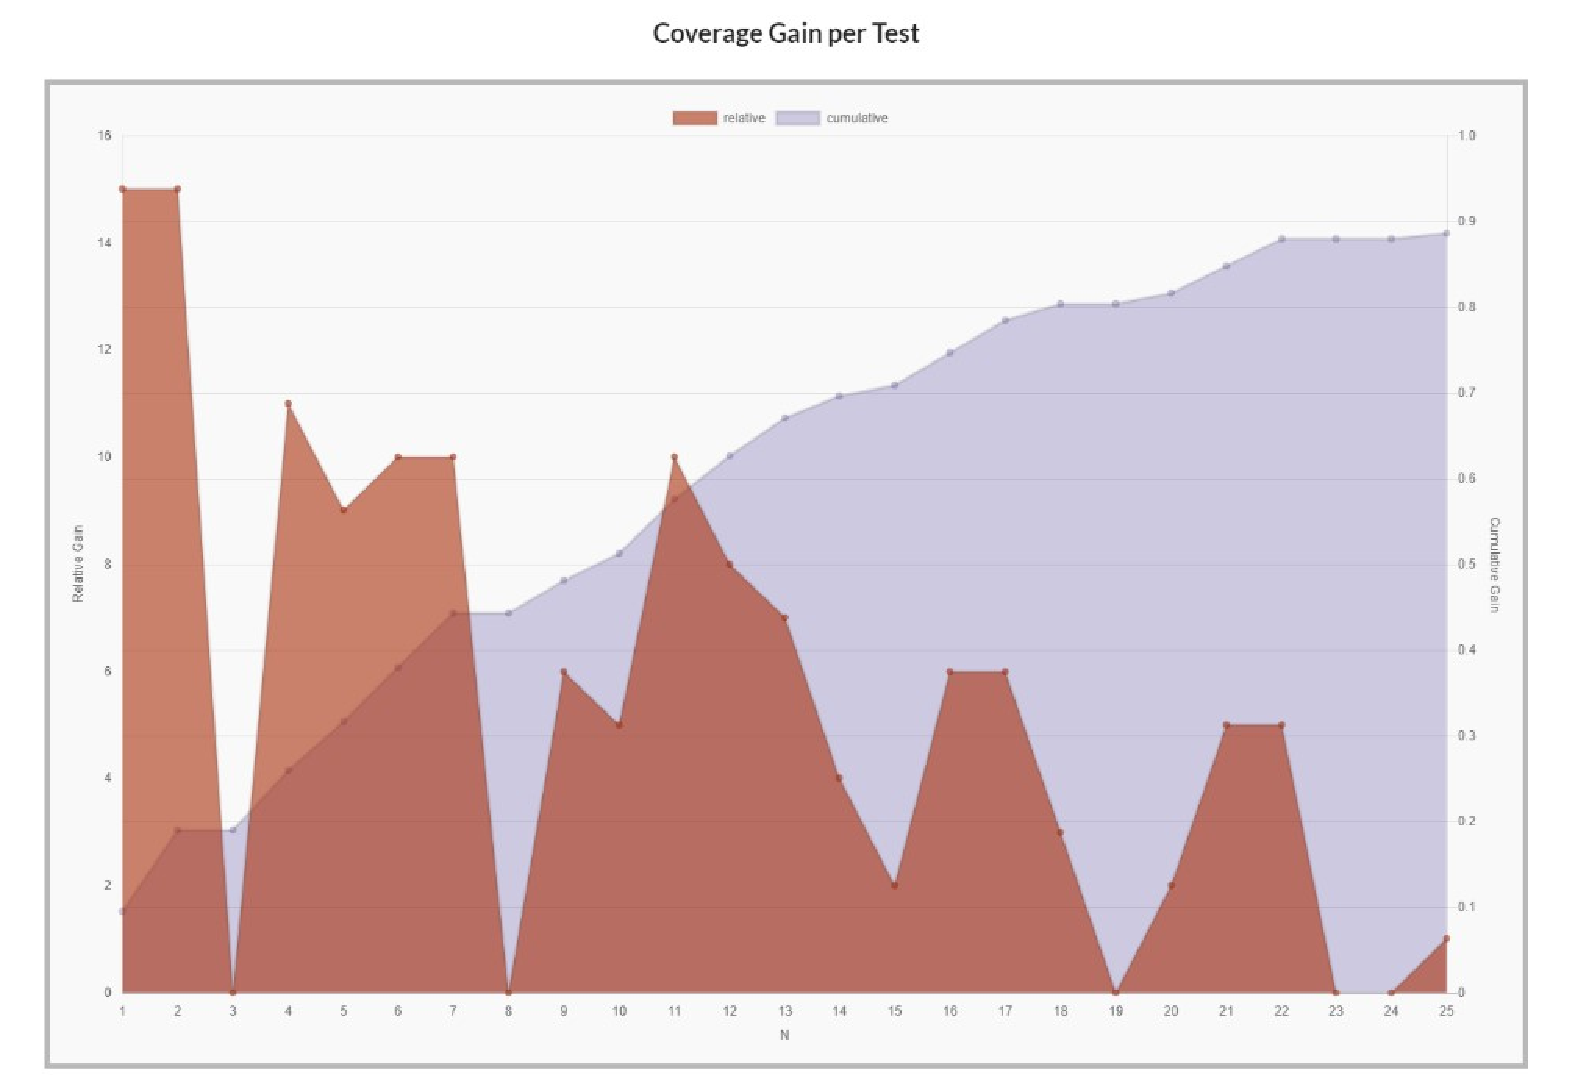
\includegraphics[width=0.50\textwidth,]{coverageGainPerTest_withConstraints.pdf}
		\caption{Constraints applied to Figure~\ref{fig:coverageGainPerTest}}
		\label{fig:coverageGainPerTest_withConstraints}
	\end{figure}

	Introducing the boolean parameters for sequencing and the constraints did not impact the number of test cases; the final number was still 19.
	Figure~\ref{fig:CompletenessCoverage} shows 2-way and 3-way completeness coverage using CCM \todo{reference to CCM}. 
	For the 2-way covering array, completeness coverage of 2-way combinations was found to be as such: 100\% of 2 tuples covered to 100\%. 
	To elaborate, of the 158 2-way tuples, all are included in the covering array for this test suite to have full pairwise / 2-way coverage.
	For reference, 3-way completeness coverage is also shown: 25\% of 3-way combinations are covered to 100\%, 50\% of 3-way combinations were covered to 95\%.
	To elaborate, of the 629 3 tuples, 25\% of them provide 3-way coverage at 100\%, 50\% of them provide 95\% 3-way coverage and so on.

	The significance and the impact of minimum t-way coverage on branch coverage conditions in the code is discussed in the paper \todo{insert reference} Measuring and Specifying Combinatorial Coverage of Test Input Configurations.
	Label M as the minimum 2-way coverage; i.e., the lowest proportion of settings covered for all t-way combinations of variables.
	For example, 2-way combinations of binary variables have four possible settings:00, 01, 10, 11.
	Some variable pairs may have all four settings covered, but others may have less.
	M is the smallest proportion of coverage among all of the t-way variable combinations.
	M is also viewable as the rightmost line in the coverage strength meters.

	At a small scale this technique was effective; for 3 parameters, the 6 sequences were possible to be incorporated into the input parameter model without increasing the number of tests. 
	Also the cost of creating the constraint logic was low since only two constraints had to be written.
	However, it can be observed that with a higher number of parameters this approach can get less cost effective. 
	The team has not encountered such a problem yet and is looking forward to the challenge in a future study.
	
	\begin{figure}[!h]
		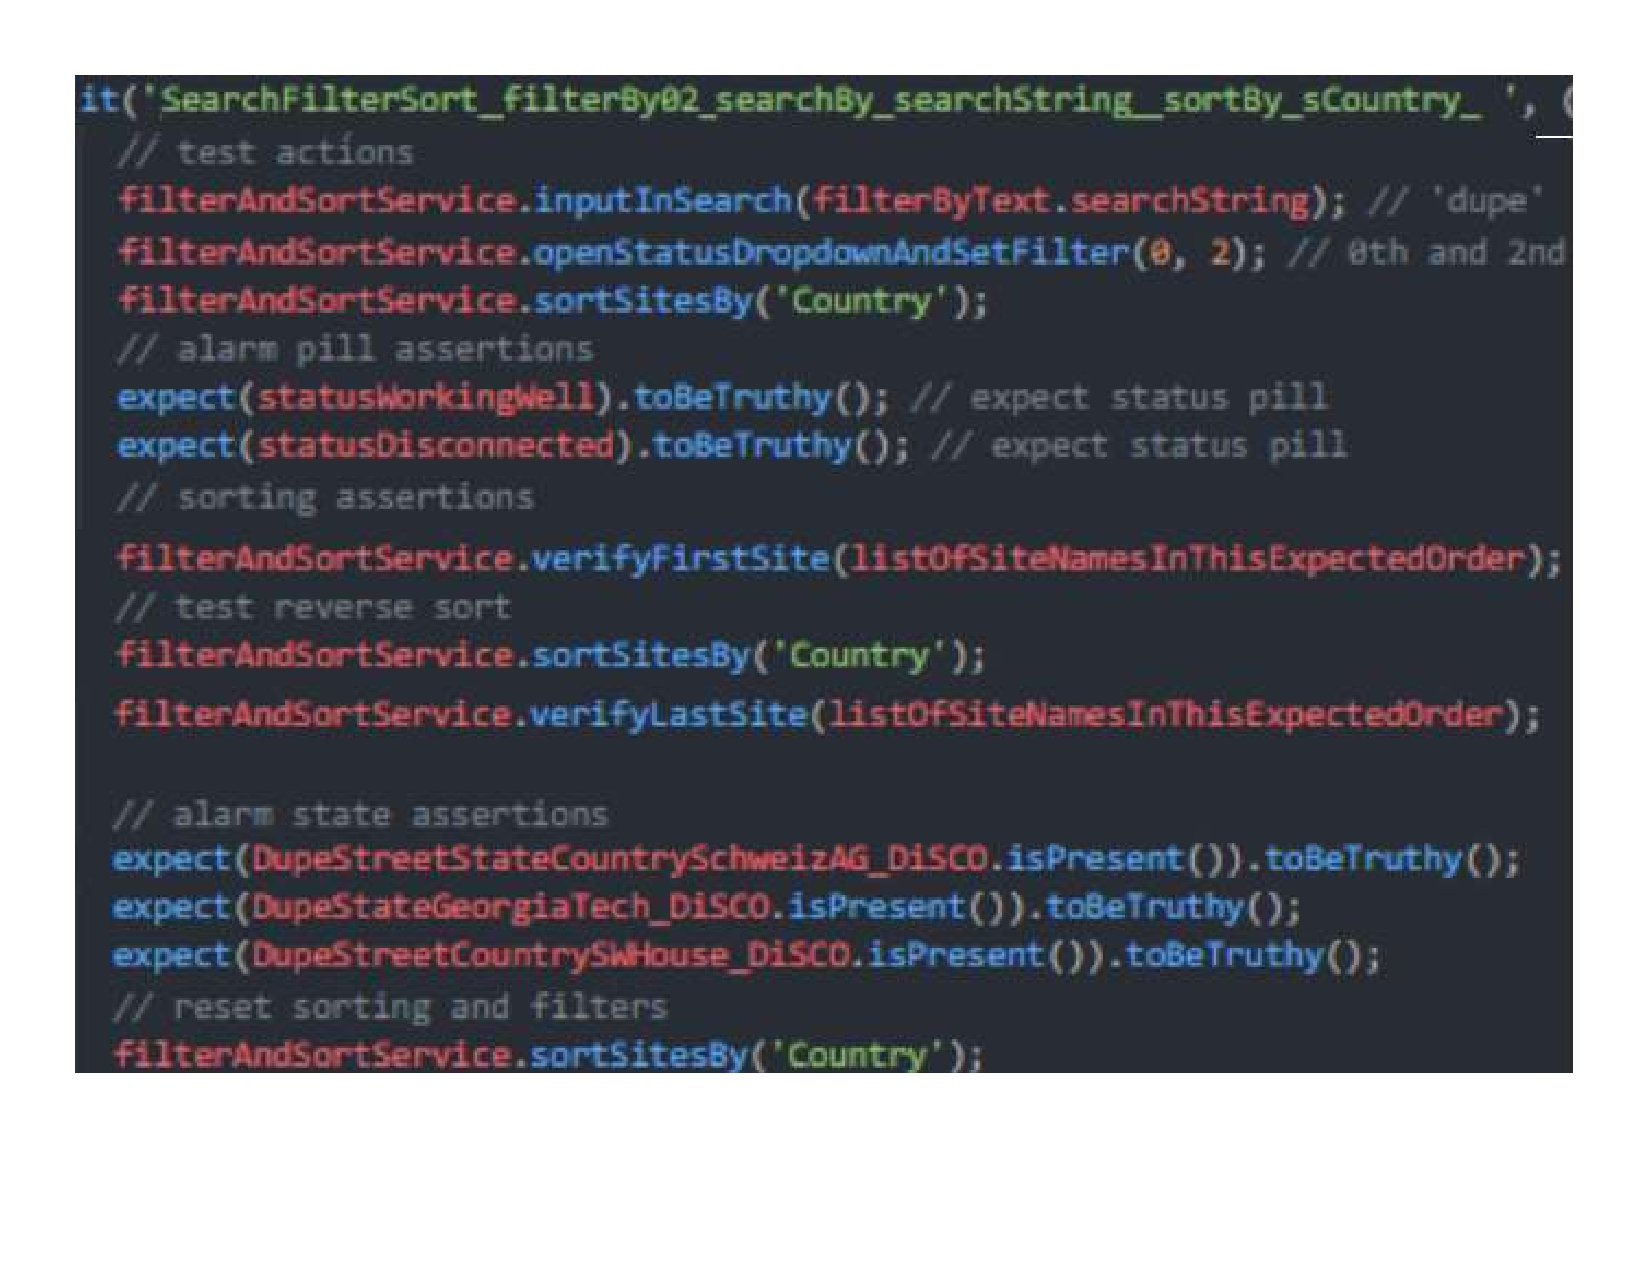
\includegraphics[width=0.50\textwidth,]{sortingTestCode.pdf}
		\caption{One of the 19 automated Protractor tests in site filtering test suite}
		\label{fig:sortingTestCode}
	\end{figure}

	To conclude this sections, Figure~\ref{fig:sortingTestCode} displays autormated Protractor test code for one of the 19 tests.
	The test actions are in the sequence \textit{search} (by text string), set \textit{site status} dropdown and \textit{sort} (by country). 
	The 3 functions execute these actions.
	In turn, status pills are verified, verifying site status.
	Following that, the sorting and reverse sorting of the sites are verified.
	Finally, the test oracle is verified to verify that the sites that are displayed in the filter.
		
	\begin{figure*}[!hb]
		\centering
			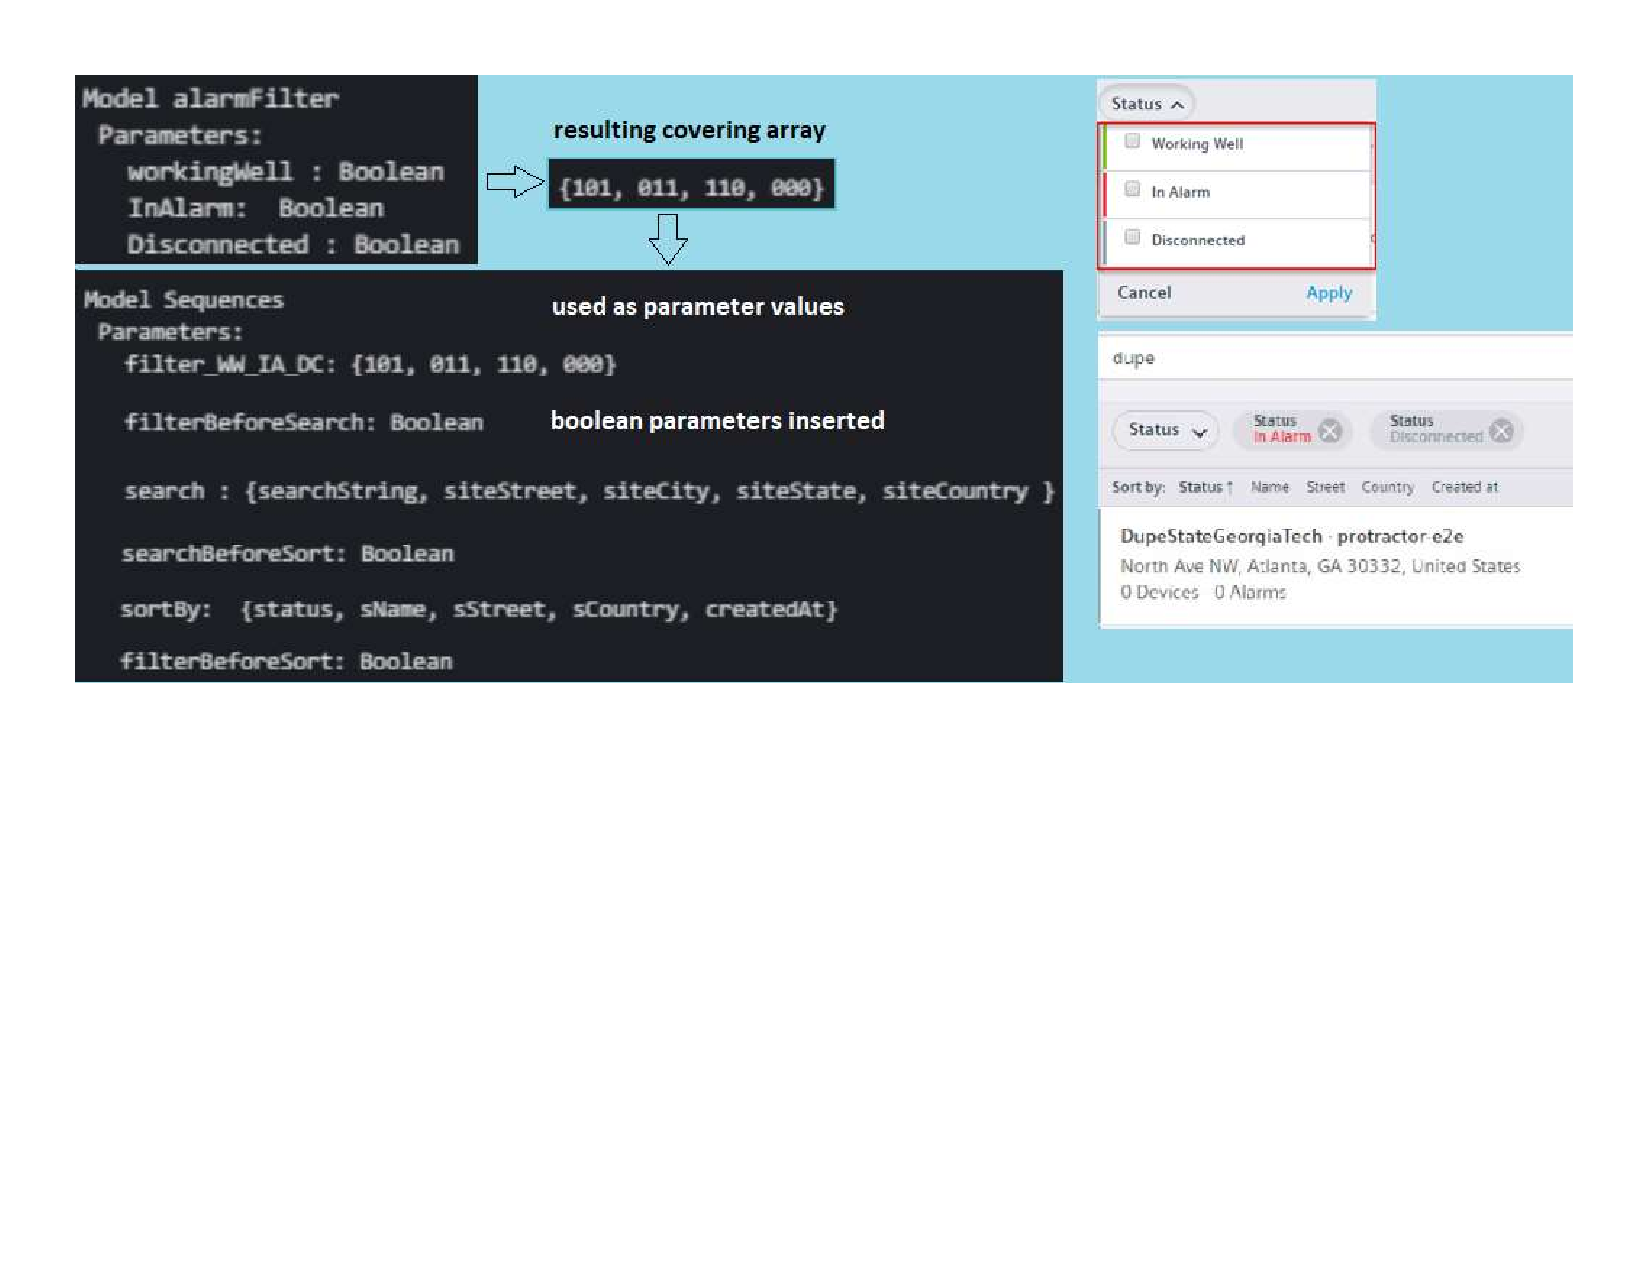
\includegraphics[width=0.95\textwidth,]{siteFilterModel.pdf}
			\caption{CT model of site filtering in CTWedge \& screen capture}
			\label{fig:siteFilterModel}
	\end{figure*}
	

\section{Conclusion and future work}
	
The initial challenge in this study was how to best test EEO configurations in the most efficient manner.
During the study it became apparent that the methods applied can be used to test any system where the parameter groups for
the Combinatorial Input Parameter Model (IPM) are not simultaneously available, and instead may appear sequentially.
Future work on this front may incorporate system test ideas where each seed (in the SBA method) or different color (in the IBM method) being a different module of functionality.

\textbf{Acknowledgments.}
This research was carried out in the context of Austrian COMET K1
program and publicly funded by the Austrian Research Promotion Agency
(FFG) and the Vienna Business Agency (WAW).

\bibliographystyle{IEEEtran}
\bibliography{cloud}

\end{document}
